\documentclass[AMS,STIX1COL]{WileyNJD-v2}
%\documentclass[AMS]{WileyNJD-v2}
\usepackage{graphicx,times,verbatim,amsmath,amsthm}
%\usepackage{graphicx,times,verbatim,amsmath,amssymb,amsthm}
\usepackage{amsmath,amsfonts}
\usepackage{bbm}
\usepackage{mathtools}
\usepackage{float}  % For fixing the image in draft
\usepackage{lscape}
\usepackage[nottoc,notlot,notlof]{tocbibind}
\newcommand{\block}[1]{
  \underbrace{\begin{matrix}1 & \cdots & 1\end{matrix}}_{#1}
}
%\newtheorem{theorem}{Theorem}[section]
%\newtheorem{lemma}[theorem]{Lemma}
%\newtheorem{corollary}[theorem]{Corollary}
%\newtheorem{proposition}[theorem]{Proposition}
%\newtheorem{definition}[theorem]{Definition}
%\newtheorem{remark}[theorem]{Remark}
%\newtheorem{condition}[theorem]{Condition}
%\newtheorem{assumption}[theorem]{Assumption}
%\newtheorem{property}[theorem]{Property}
%\newtheorem{result}[theorem]{Result}
%\newtheorem{example}[theorem]{Example}

\DeclarePairedDelimiter\ceil{\lceil}{\rceil}
\DeclarePairedDelimiter\floor{\lfloor}{\rfloor}

\articletype{Article Type}%

\received{13 May 2019}
\revised{13 May 2019}
\accepted{13 May 2019}

\raggedbottom

\begin{document}

\title{Factor Analysis on Citations, Using a Combined Latent and Logistic Regression Model}

\author[1]{Namjoon Suh}
\author[1]{Xiaoming Huo*}
\author[2]{Eric Heim}
\author[2]{Timothy Van Slyke}
\author[2]{Lee Seversky}

\authormark{Namjoon Suh \textsc{et al}}

\address[1]{\orgdiv{School of Industrial and Systems Engineering}, \orgname{Georgia Institute of Technology}, \orgaddress{755 Ferst Dr, Atlanta, \state{GA}, \country{USA}}}

\address[2]{\orgdiv{Information System Division (AFRL/RIS)}, \orgname{the Air Force Research Laboratory}, \orgaddress{Department of the Air Force, Air Force Materiel Command, AFRL/RIK - Rome, 26 Electronic Parkway, Rome,  \state{New York}, \country{USA}}}


\corres{*Xiaoming Huo, Georgia Institute of Technology, \email{huo@gatech.edu}}

\presentaddress{755 Ferst Dr, Atlanta, GA, USA.}

\abstract[Summary]{We propose a combined model, which integrates the latent factor model and the logistic regression model, for the citation network.
It is noticed that neither a latent factor model nor a logistic regression model alone is sufficient to capture the structure of the data.
The proposed model has a latent (i.e., factor analysis) model to represents the main technological trends (a.k.a., factors), and adds a sparse component that captures the remaining ad-hoc dependence.
Parameter estimation are carried out through the construction of a joint-likelihood function of edges and properly chosen penalty terms.
The convexity of the objective function allows us to develop an efficient algorithm, while the penalty terms push towards a low-dimensional latent component and a sparse graphical structure.
Simulation results show that the proposed method works well in practical situations.
The proposed method has been applied to a real application, which contains a citation network of statisticians (Ji and Jin, 2016 \cite{ji2016coauthorship}).
Some interesting findings are reported.
}

\keywords{citation network, matrix decomposition, latent variable model, logistic regression model, convex optimization, ADMM}

\jnlcitation{\cname{%
\author{Suh Namjoon.},
\author{Xiaoming Huo},
\author{Eric Heim},
\author{Timothy Van Slyke}, and
\author{Lee Seversky}} (\cyear{2019}),
\ctitle{Citation network}, \cjournal{journal.}, \cvol{2019;00:1--6}.}
\maketitle
\footnotetext{\textbf{Abbreviations:} fused factor analysis and logistic graphical models, ADMM, network model}

\section{Introduction}
\label{sec:intro}
We study a citation network, where each node (i.e., item) can be a technical report or a publication.
A node may cite another node.
Associated with a pair of nodes $i$ and $j$, we denote a binary random variable $X_{ij}$, where $1 \le i,j \le n$ and $n$ is the total number of nodes.
We have $X_{ij}=1$ if and only if either node $i$ cites node $j$ or vice versa; otherwise $X_{ij}=0$.
For each node $i$, we assume that there is an associated binary vector $f_{i} \in \mathbb{R}^K$, such that the $k$th entry of $f_{i}$, $f_{ik} = 1$, if and only if node $i$ is related to topic (i.e., factor) $k, 1\le k \le K$.
Here $K$ is the total number of underlying topics (i.e., factors, or trends).
We assume a logistic model for $X_{ij}$'s: for $1\le i,j \le n$,

\begin{equation}
\label{eq:logistic01}
\mathbb{P}(X_{ij}=1) = \frac{e^{\alpha + f_i^T D f_j }}{1 + e^{\alpha + f_i^T D f_j }},
\end{equation}
where $\alpha \in \mathbb{R}$ is a parameter and matrix $D \in \mathbb{R}^{K \times K}$ is a diagonal matrix: $D = \mbox{diag}\{d_{1},d_{2},\ldots,d_{K}\}$.
We assume $d_{ii} > 0$ for $1 \le i \le K$.
Another way to put \eqref{eq:logistic01} is
\begin{equation}
\label{eq:logistic02}
\mathbb{P}(X_{ij}=1) = \frac{\exp\left(\alpha + \sum_{k=1}^K f_{ik}f_{jk}d_{k} \right)}{1 + \exp\left(\alpha + \sum_{k=1}^K f_{ik}f_{jk}d_{k} \right)}.
\end{equation}
A justification of the above model is that when both node $i$ and node $j$ are related to topic $k$, they have a higher chance to cite one way or the other.
We have assumed a common strengthen coefficient $d_k$ ($1\le k \le K$) for factor $k$, despite different nodes.
We denote a matrix $F = \{f_1, f_2, \ldots, f_n\} \in \mathbb{R}^{K \times n}$.
Each column $i$ in matrix $F$ contains the factor loadings associated with the node $i$ ($1\le i \le n$).
Given the diagonal matrix $D$ and the factor loading matrix $F$, we assume that $X_{ij}$'s are independent; therefore we have the total conditional probability function as follows:
\begin{equation}
\label{eq:logistic03}
\mathbb{P}(\{X_{ij}, 1\le i,j \le n\})
= \prod_{1\le i<j \le n} \mathbb{P}(X_{ij})
= \prod_{1\le i<j \le n}  \frac{e^{X_{ij}(\alpha + f_i^T D f_j) }}{1 + e^{\alpha + f_i^T D f_j }},
\end{equation}
where $\mathbb{P}(X_{ij})$ is given in \eqref{eq:logistic02}.
The last equation holds because $X_{ij}$ only takes binary (i.e., $0$ or $1$) values.
Recall that the dot product of two matrices with same dimensionality, $A,B\in \mathbb{R}^{a \times b}$, is defined as $A\bullet B=\mbox{trace}(A^T B) = \sum_{i=1}^a\sum_{j=1}^b a_{ij}b_{ij}$.
The above \eqref{eq:logistic03} can be further rewritten as
\begin{equation}
\label{eq:logistic04}
\mathbb{P}(\{X_{ij}, 1\le i,j \le n\})
= \frac{\exp\left(\alpha \sum_{1\le i< j\le n}X_{ij} +\frac{1}{2} X \bullet (F^T D F)\right)}{\prod_{1\le i<j \le n}  1 + e^{\alpha + f_i^T D f_j }},
\end{equation}
where we assume $X_{ii}=0$ for all $i$ ($1\le i \le n$) and $X_{ij} = X_{ji}$ for all $i$ and $j$ ($1\le i,j \le n$), i.e., the matrix $X$ is symmetric.
The above delivers a factor analysis model.
Various linear and nonlinear latent variable models have been studied extensively in the literature (e.g.,\cite{joreskog1969general, mcdonald2014factor,lord2008statistical, rasch1980probabilistic, harman1960modern, joreskog1970general}).

Our work is motivated from a recent work named {\emph{Fused Latent and Graphical (FLaG) model} (Chen et al, 2016, \cite{chen2016fused}).
They assume that majority of variation of responses can be accounted by low dimensional latent vector, and remaining dependent structure of responses can be explained by sparse graphical structure.
Thus, the resulting model contains a low-dimensional latent vector and a sparse conditional graph.
Their key idea is to separate these two dependent structures so that they can facilitate the statistical inference.
In our model, we also assume that there exist two dependent structures among citation edges in a network.
A low-dimensional version of the aforementioned latent vector model is largely correct and majority of the citations among the nodes are induced by these common latent vectors $f_{i}$'s (with weight coefficients $d_{i}$'s).
There is still a small remainder due to the sparse graphical component.

Though it may seem similar to Chen et al \cite{chen2016fused}, we work on a different model formulation in several aspects.
We summarize the differences as follows.
\begin{enumerate}
\item FLaG is built to analyze the Eysenck's Personality Questionnaire that consists of items designed to measure Psychoticism, Extraversion, and Neuroticism.
    So there are $p$ questions that need to be answered, and each questions fall into above three categories.
    If there are $n$ respondents to questions, we have $n$ independent data generated from same distribution.
    In our case, the observed citation network can be thought of as one realization of a random graph.

\item In FLaG model, a collection of binary responses for each question in the questionnaire follows a joint distribution, which is a combination of the Item Response Theory (IRT) model and the Ising model.
    We model the citation edges among papers as random variables, whose dependent structure is characterized by the combination of the Latent Factor Analysis model and the Sparse Graphical model.

\item FLaG approximates the original likelihood through constructing pseudo-likelihood function by taking advantage of conditional independence among the nodes.
    In our model, likelihood function is directly accessible due to the conditional independence among edges given parameters.
\end{enumerate}

The proposed modeling framework is also related with the analysis of decomposing a matrix into low-rank and sparse components (\cite{agarwal2012noisy,candes2011robust,chandrasekaran2010latent, zhou2010stable}).
Specifically, \cite{chandrasekaran2010latent} studies statistical inference of a multivariate Gaussian model whose precision matrix admits the form of a low-rank matrix plus a sparse matrix.
The inference and optimization of the current model are different from the aforementioned cases.
We will construct a regularized-likelihood function, based on which estimator will be proposed for simultaneous model selection and parameter estimation.
The objective function in the optimization problem for the regularized estimator is convex, for which we will develop an efficient algorithm through the alternating direction method of multiplier (ADMM, \cite{boyd2011distributed, gabay1975dual, glowinski1975solution}).

The rest of the paper is organized as follows.
In Section \ref{sec:model-form}, we will give a presentation on how to build a model, which can encode both the latent dependent structure due to the common topics and the remaining sparse ad-hoc dependent structure.
In Section \ref{sec:estimate}, we will discuss the assumptions in our model and penalization on likelihood function that is constructed in Section \ref{sec:model-form}.
In Section \ref{sec:theorem}, we provide a non-asymptotic error bound of the estimator.
Section \ref{sec:compute} gives the detailed procedure on how to compute the estimator of the optimization problem that is formulated in Section \ref{sec:estimate}.
In Section \ref{sec:Num-anal}, we will present simple numerical experiments on synthetic data, and application of our model on real citation network of statisticians.
We finally conclude this work in Section \ref{sec:Con} with several open questions and some directions for future research.

\section{Model Formulation}
\label{sec:model-form}

Recall the following graphical model that was established in \eqref{eq:logistic04}, which is essentially a factor model (latent variable model):
$$
\mathbb{P}\left(\{X_{ij}, 1\le i,j \le n\}\right)
= \frac{\exp\left(\alpha \sum_{1\le i< j\le n}X_{ij} +\frac{1}{2} X \bullet (F^T D F)\right)}{\prod_{1\le i<j \le n}  1 + e^{\alpha + f_i^T D f_j }},
$$
where
$X_{ij}, 1\le i,j \le n$, are binary random variables indicating either node $i$ cites node $j$ or vice versa,
matrix $X = \{X_{ij}\} \in \mathbb{R}^{n \times n}$ is symmetric with diagonal entries all being equal to zero,
factor loading matrix $F = [f_1,f_2,\ldots,f_n]\in \mathbb{R}^{K\times n}$ records the relation between nodes and the underlying topics, $F^T$ is the transpose of $F$,
and matrix $D \in \mathbb{R}^{K \times K}$  is diagonal with entries being the weight coefficients of factors.

The above specifies a latent model (or equivalently a factor model).
We now describe a graphical model as follows.
The graphical model will complement the latent model by characterizing links that are not interpretable via common factors.
For the aforementioned binary random variable $X_{ij}$, $1\le i,j \le n$, we define
\begin{equation}
\label{eq:logistic05}
\mathbb{P}(X_{ij}=1) = \frac{e^{\alpha' + S_{ij} }}{1 + e^{\alpha' + S_{ij} }},
\end{equation}
where $S_{ij} \in \mathbb{R}$, for $1\le i,j \le n$, denotes the relation between nodes $i$ and $j$.
Note that the matrix $S$ is introduced to capture the ad-hoc links in the graph.
If we have $S_{ij}\leq0$, then it is less likely to have a citational relationship between nodes $i$ and $j$.
On the other hand, if $S_{ij}>0$, then it is more likely to have a citation link between nodes $i$ and $j$.
Here parameter $\alpha' \in \mathbb{R}$ plays the same role as parameter $\alpha$ does in model \eqref{eq:logistic01}.
Denote the matrix $S = \{S_{ij}, 1\le i,j \le n \} \in \mathbb{R}^{n \times n}$.
Assume that given the matrix $S$, the binary random variables
$X_{ij}$'s are independent;
consequently, we have the total conditional probability function as follows:
\begin{eqnarray}
\mathbb{P}(\{X_{ij}, 1\le i,j \le n\})
&=& \prod_{1\le i<j \le n} \mathbb{P}(X_{ij}) \nonumber \\
&=& \prod_{1\le i<j \le n}  \frac{e^{X_{ij}(\alpha' + S_{ij}) }}{1 + e^{\alpha' + S_{ij} }} \nonumber \\
&=& \frac{\exp\left(\alpha' \sum_{1\le i< j\le n}X_{ij} +\frac{1}{2} X \bullet S\right)}{\prod_{1\le i<j \le n}  1 + e^{\alpha' + S_{ij} }}.
\label{eq:logistic06}
\end{eqnarray}
Recall that we have assumed that $X_{ii}=0$ for all $i$ ($1\le i \le n$) and $X_{ij} = X_{ji}$ for all $i$ and $j$ ($1\le i,j \le n$), i.e., the matrix $X$ is symmetric.
In the combined model, we integrate \eqref{eq:logistic04} and
\eqref{eq:logistic06} to render the joint conditional probability function as follows:
\begin{eqnarray}
\label{eq:logistic07}
\mathbb{P}(X \mid \alpha,  F, D, S)
&=&  \prod_{1\le i<j \le n}
\frac{e^{X_{ij}(\alpha + S_{ij} + f_i^T D f_j) }}{1 + e^{\alpha + S_{ij}+ f_i^T D f_j}} \nonumber \\
&=& \frac{\exp\left(\alpha \sum_{1\le i< j\le n}X_{ij} +\frac{1}{2} X \bullet (F^T D F) +\frac{1}{2} X \bullet S\right)}{\prod_{1\le i<j \le n}  \left(1 + e^{\alpha + f_i^T D f_j +S_{ij}}\right) }.
\end{eqnarray}


\section{Estimation}
\label{sec:estimate}
Note that in the model \eqref{eq:logistic07}, the log-likelihood function has the form as follows:
\begin{eqnarray}
\label{eq:logistic08}
\mathbb{L}(\alpha,  F, D, S; X)
&=& \alpha \sum_{1\le i< j\le n}X_{ij} +\frac{1}{2} X \bullet (F^T D F) +\frac{1}{2} X \bullet S \\
&& -\sum_{1\le i<j\le n} \log \left(1 + e^{\alpha + f_i^T D f_j +S_{ij} }\right). \nonumber
\end{eqnarray}

If we consider maximizing the above log-likelihood function,
we will encounter several technical issues that are described below.
\begin{enumerate}
\item We would like the matrix $S \in \mathbb{R}^{n \times n}$ to have as many zero entries as possible; i.e., matrix $S$ is {\it sparse.}

\item There is an identifiability issue with the formation $F^T D F$.
More specifically, let $P \in \mathbb{R}^{K \times K}$ be a signed permutation matrix, then we have $P^T P = I_n$, where $I_n \in \mathbb{R}^{K \times K}$ is the identity matrix.
Notice that matrix $F' = PF$ is also a factor loading matrix, and
matrix $D' = P D P^T$ is still a diagonal matrix;
we have
$$
F^T D F = F^T P^T P D P^T P F = (F')^T D' F',
$$
i.e., the choice of $F$ and $D$ is not unique.

\item We would like the number of nonzeros in each column of $F$ to be small, reflecting that each node is associated with a small number of underlying topics.

\item Overall, the rank of matrix $F^T D F$ cannot be larger than $\min\{n,K\}$.
With the application that we have in mind, in this paper, we assume that $K$ is much smaller than $n$.

\item To ensure the separation of matrices $\alpha\mathbbm{1}\mathbbm{1}^T$ and an arbitrary matrix $L$, we assume that the eigen-vector of $L$ is centered, that is,
\[
    JLJ = L \quad \mbox{where} \quad
    J=I_{n}-\frac{1}{n}\mathbbm{1}\mathbbm{1}^T,
\]
where $\mathbbm{1}$ denotes a $n$-dimensional vector whose entries are all $1$'s. If we have $L=F^TDF$, this condition uniquely identifies $F$ up to a common orthogonal transformation of its columns.

\end{enumerate}


Directly maximizing the objective function in \eqref{eq:logistic08} is not going to be an easy task.
Following the approaches that were mentioned in Introduction, we propose to relax $F^T D F$ to $L$, where $L$ is a low rank matrix.
Consequently, the log-likelihood function in \eqref{eq:logistic08} can be rewritten as
\begin{eqnarray}
\label{eq:logistic09}
\mathbb{L}_n(\alpha,  L, S; X)
&=& \alpha \sum_{1\le i< j\le n}X_{ij} +\frac{1}{2} X \bullet L +\frac{1}{2} X \bullet S \\
&& -\sum_{1\le i<j\le n} \log \left(1 + e^{\alpha + L_{ij} +S_{ij}}\right). \nonumber
\end{eqnarray}


We propose a penalized likelihood estimation approach as follows:
\begin{eqnarray}
\label{eq:logistic10}
(\hat{\alpha}, \widehat{L}, \widehat{S})
= \mbox{arg min}_{\alpha, L, S} \left\{
-\frac{1}{n} \mathbb{L}_n(\alpha,  L, S; X) + \gamma \|S\|_1
+ \delta \|L\|_\ast\right\},
\end{eqnarray}
where $\gamma>0$ and $\delta>0$ are algorithmic parameters whose values will be discussed later,
the $L_1$ norm of matrix $S$ is defined as $\|S\|_1 = \sum_{i\neq j} |S_{ij}|$ (Note that we do not penalize the diagonal entries of $S$), and nuclear norm of matrix $L$ is defined as $\|L\|_\ast = {\mbox{trace}\sqrt{(L^T L)}}$.
Recall that both $S$ and $L$ are symmetric matrices.
The entries of matrix $S$ can either be positive or negative.
Note that we have imposed the diagonal entries of the matrix $X$ to be zeros.
Given that $L = F^T D F$ where matrix $D$ is diagonal with nonnegative diagonal entries, it is easy to see that matrix $L$ is positive semidefinite; which consequently leads to $\|L\|_\ast = \mbox{trace}(L)$, which is a linear functional to the matrix $L$.
The nuclear norm of $L$ mimicks the number of nonzero eigenvalues of $L$, which is the same as the rank
of $L$.
The regularization based on the nuclear norm was proposed in \cite{fazel2001rank}
and its statistical properties are studied in \cite{bach2008consistency}.

After we have obtained $\widehat{S}$ in \eqref{eq:logistic10}, we can uncover the graphical model by investigating non-zero entries in $\widehat{S}$.
On the other hand when we have calculated $\widehat{L}$, we may not be able to find binary matrix $F$ and nonnegative diagonal matrix $D$ such that $\widehat{L} = F^T D F.$
This is the price we have to pay for an amenable computational approach.
The rank of estimated $\widehat{L}$ will be our estimate of the number of factors (i.e., the number of underlying common topics).
For the issue on assigning the community membership of each node $i$, we will discuss this later in Section \ref{sec:Num-anal}.

\section{Non-asymptotic error bound of the estimator}
\label{sec:theorem}
In this section, we focus on investigating the behaviour of non-asymptotic error bound of our estimator in the context where the number of papers in a network is explicitly tracked. We are interested in solving the following optimization problem :
\begin{equation}\label{eq:Modified}
\min\limits_{\alpha \in R, S = S^T \atop L \succcurlyeq 0}
-\frac{1}{n} \log \prod_{1\le i,j\le n}\frac{\exp\left(X_{ij}\left(\alpha+
L_{ij}+S_{ij}\right)\right)}{1+\exp\left(\alpha+
L_{ij}+S_{ij}\right)} + \delta \|L\|_\ast + \gamma \|S\|_1
\end{equation}

%Astute readers might notice the slight difference of the first term in objective function between (\ref{eq:logistic10}) and (\ref{eq:Modified}).
For the convenience of theoretical investigation, we slightly modify the first term in the objective function summing over all $(i,j)$ pairs.
After scaling, due to symmetry of $X$,$L$, and $S$, the only difference between (\ref{eq:logistic10}) and (\ref{eq:Modified}) is in the inclusion of terms in diagonal pairs $(i,i),\forall i=1,\dots,n$.
%the first term in the objective function in (\ref{eq:Modified}) sums over all $(i,j)$ pairs.
This slight modification leads to neither theoretical consequence nor noticeable difference in practice.
Let ($\widehat{\alpha},\widehat{L},\widehat{S}$) be the solution to (\ref{eq:Modified}), and ($\alpha^{*},L^{*},S^{*}$) be the ground truth, which governs the data generating process.
Let $\widehat{\Theta}$ and $\Theta^{*}$ be defined respectively as $\widehat{\Theta} = \widehat{\alpha}\mathbbm{1}\mathbbm{1}^T+\widehat{L}+\widehat{S}$ and $\Theta^{*} = \alpha^{*}\mathbbm{1}\mathbbm{1}^T+L^{*}+S^{*}$.
And denote the error term for each parameter as $\widehat{\Delta}^{\Theta} = \widehat{\Theta}-\Theta^{*},
\widehat{\Delta}^{\alpha} = \widehat{\alpha}-\alpha^{*},
\widehat{\Delta}^L = \widehat{L}-L^{*},
\widehat{\Delta}^S = \widehat{S}-S^{*}.$
Throughout the discussion, let $P^{*}=\big\{\frac{\exp(\Theta_{ij}^{*})}{1+\exp(\Theta_{ij}^{*})}\big\}_{1 \leq i,j \leq n} \in \mathbb{R}^{n \times n}$.
We then impose several assumptions for theoretical guarantees of our estimator.

\begin{assumption}(\textbf{Strong convexity})  \label{Ass:1}
For any $\Theta \in \mathbb{R}^{n\times n}$, define the log-likelihood in (\ref{eq:Modified}), $h(\Theta) = -\frac{1}{n}\sum_{i,j} \big\{ X_{ij}\Theta_{ij} - \log(1+\exp(\Theta_{ij})) \big\}$.We assume that $h(\Theta)$ is $\tau$-strongly convex in a sense that lowest eigenvalue of Hessian matrix of the log-likelihood function is bounded away from zero ($\tau > 0$):
\[
\nabla^{2}h(\Theta) = \mbox{diag}\Big(\mbox{vec}\Big(\frac{\exp(\Theta)}{n(1+\exp(\Theta))^{2}}
\Big)\Big) \succcurlyeq \tau I_{n^{2} \times n^{2}}
\]
For any vector $a$, $\mbox{diag}(a)$ is the diagonal matrix with elements of $a$ on its diagonal.
For any matrix $B=[b_1,\dots,b_n]\in\mathbb{R}^{n \times n}$, $\mbox{vec}(B)\in\mathbb{R}^{n^2}$ is obtained by stacking $ b_1,\dots, b_{n}$ in order.
For any square matrix $A$ and $B$, we have $ A \succcurlyeq B $ if and only if matrix $A-B$ is positive semi-definite.
\end{assumption}

\begin{assumption} (\textbf{Identifiability of $\alpha\mathbbm{1}\mathbbm{1}^T$ and L, Spikiness of L}) \label{Ass:2}
To ensure the identifiability of $\alpha\mathbbm{1}\mathbbm{1}^T$ and L, we assume that the latent variables are centered, that is $JL=L$, where $J=I_{n}-\frac{1}{n}\mathbbm{1}\mathbbm{1}^T$, where $\mathbbm{1}$ denotes all one vector in $\mathbb{R}^{n}$. We impose a spikiness condition $\|L\|_{\infty}\leq\frac{\kappa}{\sqrt{n \times n}}$ on L, to ensure the separation of L and S matrix \cite{agarwal2012noisy}. We would also like to note that the constraint $|\alpha|\leq C\kappa$, for an absolute constant $C$, is included partially for obtaining theoretical guarantees.
\end{assumption}

With these assumptions, we present the behavior of non-asymptotic error bound of our estimator through the following theorem. In our result, we measure error using squared Frobenius norm summed across three matrices:
\[
    e^{2}(\widehat{\alpha}\mathbbm{1}\mathbbm{1}^T,\widehat{L},\widehat{S})
    :=\|\widehat{\Delta}^{\alpha}\mathbbm{1}\mathbbm{1}^T\|_{F}^{2} + \|\widehat{\Delta}^{L}\|_{F}^{2} + \|\widehat{\Delta}^{S}\|_{F}^{2}
\]

\begin{theorem} \label{Th:th1}
Under the assumptions \ref{Ass:1} and \ref{Ass:2},
if we solve the convex problem (\ref{eq:Modified}) with a pair of regularization parameter $(\delta,\gamma)$ satisfying
\begin{align} \label{eq:49}
\delta \geq 2\|\frac{1}{n}(X-P^{*})\|_{op} \quad and \quad \gamma \geq 2\|\frac{1}{n}(X-P^{*})\|_{\infty}+4\kappa\tau\bigg(\frac{Cn+1}{n} \bigg),
\end{align}
then there exist universal constants $c_{j}$, j = 1,2,3,  for all integers $k = 1,2,...,n$, and $s = 1,2,...,n^{2}$, and we have the following upper bound on $e^{2}(\widehat{\alpha}\mathbbm{1}\mathbbm{1}^T,\widehat{L},\widehat{S})$
\begin{align}
    e^{2}(\widehat{\alpha}\mathbbm{1}\mathbbm{1}^T,\widehat{L},\widehat{S}) \leq
    \underbrace{c_{1}\frac{\delta^{2}}{\tau^{2}}}
    _{\mathcal{K}_{\alpha^*}} +
    \underbrace{c_{2}\frac{\delta^{2}}{\tau^{2}}
    \bigg\{k + \frac{\tau}{\delta}\sum_{j=k+1}^{n}\sigma_{j}(L^{*})\bigg\}}_{\mathcal{K}_{L^*}} +
    \underbrace{c_{3}\frac{\gamma^{2}}{\tau^{2}}
    \bigg\{s + \frac{\tau}{\gamma}\sum_{(i,j) \notin M}|S^*_{ij}|\bigg\}}_{\mathcal{K}_{S^*}},
\end{align}
where $M$ is an arbitrary subset of matrix indices of cardinality at most s.
\end{theorem}

We would first like to note that the result presented in Theorem \ref{Th:th1} can be thought of as an extension to Theorem $1$ presented in paper \cite{agarwal2012noisy} to a generalized linear model.
Our work considers a logistic loss function whose parameters are characterized by a sparse matrix plus a low rank matrix, whereas Agarwal, et al.\cite{agarwal2012noisy} work on a quadratic loss of a noisy realization of a linear transformation of sum of a low rank matrix and a sparse matrix.
We show that similar proof techniques can be applied in our case, giving us similar results.
%Detailed descriptions of each terms in bound are elaborated in paper \cite{agarwal2012noisy}.

Result of the Theorem \ref{Th:th1} provides a family of upper-bounds, one for each indexed by a specific choice of model subspace $M$, and rank parameter $k$, helping us to understand the behavior of our proposed estimator both in practice and in ideal cases. In real-world, large scale citation network analysis, it is difficult to expect network with $L^*$ matrix with exactly $k(\ll n)$ non-zero eigenvalues, but with a matrix $L^*$ with approximately low rank.
In this case, our theorem provides the intuition on the rate on how fast the error bound $\mathcal{K}_{L^*}$ will grow.
In ideal cases where $L^*$ is an exact low rank matrix with rank $k$ (i.e., $rank(L^*)=k$) and $S^*$ is a sparse matrix, which lies within model subspace $M$ (i.e., $|supp(S^*)|=s$), we can easily verify ``\emph{approximation error}'' terms in $\mathcal{K}_{L^*}$ (i.e., $\tau\sum_{j=k+1}^{n}\sigma_j(L^*)$) and in $\mathcal{K}_{S^*}$ (i.e., $\tau\sum_{(i,j)\notin M}|S_{ij}^*|$) disappear, giving us Frobenius error bound as follows:
\[
    e^{2}(\hat{\alpha}\mathbbm{1}\mathbbm{1}^T,\widehat{L},\widehat{S}) \lesssim \delta^2(k+1)+\gamma^2s
\]
where $\lesssim$ denotes that we ignore constant factors.

\section{Computation}
\label{sec:compute}

We propose a method that takes advantage of the special structure
of the $L_1$ and the nuclear norm by means of the
alternating direction method of multiplier (ADMM), which is a method
that has recently gained momentum.
An examination of the objective function in \eqref{eq:logistic10} unvails that
terms
\[
\alpha \sum_{1\le i< j\le n}X_{ij} +\frac{1}{2} X \bullet L +\frac{1}{2} X \bullet S
\]
are linear in $\alpha,  L$, and $S$.
The term
\[
\sum_{1\le i<j\le n} \log \left(1 + e^{\alpha + L_{ij} +S_{ij}}\right)
\]
is convex with respect to $\alpha,  L$, and $S$.
Functions $\|S\|_1$ and $\|L\|_\ast$ are known to be convex functions.
Therefore, the objective function in \eqref{eq:logistic10} is convex.
The above convex optimization problem can be solved via ADMM as follows.


\subsection{ADMM approach}
\label{sec:ADMM}
We give a review of the alternating direction method
of multiplier (ADMM).
Consider two closed convex functions
$$
f : \chi_f \to \mathbb{R} \mbox{ and } g : \chi_g \to \mathbb{R},
$$
where the domain $\chi_f$ and $\chi_g$ of functions $f$ and $g$ are closed convex subsets of $\mathbb{R}^d$, and $\chi_f \bigcap \chi_g$ is nonempty.
Both $f$ and $g$ are possibly non-differentiable.
The alternating direction method
of multiplier is an iterative algorithm that solves the following generic optimization problem:
$$
\min_{x \in \chi_f \bigcap \chi_g} \left\{f(x) + g(x) \right\},
$$
or equivalently
\begin{eqnarray}
\label{eq:admm1}
\min_{x \in \chi_f, z\in \chi_g} & \left\{f(x) + g(z) \right\}, \\
\mbox{ subject to } & x = z. \nonumber
\end{eqnarray}
To describe the algorithm, we will need the following proximal operators
\begin{itemize}
\item $\mathbf{P}_{\lambda,f}: \mathbb{R}^d \to \chi_f$ as
$$
\mathbf{P}_{\lambda,f}(v) = \mbox{arg min}_{x \in \chi_f} \left\{
f(x) + \frac{1}{2\lambda} \|x-v\|^2_2
\right\},
$$

\item and $\mathbf{P}_{\lambda,g}: \mathbb{R}^d \to \chi_g$ as
$$
\mathbf{P}_{\lambda,g}(v) = \mbox{arg min}_{x \in \chi_g} \left\{
g(x) + \frac{1}{2\lambda} \|x-v\|^2_2
\right\},
$$
where $\|\cdot\|_2$ is the usual Euclidean norm on $\mathbb{R}^d$ and $\lambda$ is a scale parameter that is a fixed positive constant.
\end{itemize}
The algorithm starts with some initial values $x^0 \in \chi_f,
z^0 \in \chi_g, u^0 (=\lambda y^0) \in \mathbb{R}^d$.
At the $(m+1)$th iteration, $(x^m, z^m, u^m)$ is updated according to the following steps until convergence
\begin{itemize}
\item Step 1: $x^{m+1} = \mathbf{P}_{\lambda,f}(z^m - u^m)$,

\item Step 2: $z^{m+1} = \mathbf{P}_{\lambda,g}(x^{m+1} + u^m)$,

\item Step 3: $u^{m+1} = u^m + x^{m+1} - z^{m+1}$.

\end{itemize}
The convergence properties of the algorithm are summarized in the following result as in \cite{boyd2011distributed}.
Let $p^\ast$ be the minimal value in \eqref{eq:admm1}.

\begin{theorem}[Boyd et al., 2011]
Assume functions $f: \chi_f \to \mathbb{R}$ and
$g: \chi_g \to \mathbb{R}$ are
closed convex functions, whose domains $\chi_f$ and $\chi_g$
are closed convex subsets of $\mathbb{R}^d$ and
$\chi_f \bigcap \chi_g \neq \emptyset$.
Assume the Lagrangian of \eqref{eq:admm1}
$$
L(x,z,y) = f(x) + g(z) + y^T(x-z)
$$
has a saddle point, that is, there exists $(x^\ast, z^\ast, y^\ast)$ (not necessarily unique) that $x^\ast \in \chi_f$ and
$z^\ast \in \chi_g$, for which
$$
L(x^\ast, z^\ast, y) \le L(x^\ast, z^\ast, y^\ast) \le
L(x, z, y^\ast), \qquad \forall x, z, y \in \mathbb{R}^d.
$$
Then the ADMM has the following convergence properties.
\begin{enumerate}
\item Residual convergence. $x^m - z^m \to 0$
as $m \to \infty$; i.e., the iterates approach feasibility.

\item Objective convergence. $f(x^m) + g(z^m) \to p^\ast$ as $m \to \infty$; i.e., the objective function of
the iterates approaches the optimal value.

\item Dual variable convergence. $y^m \to y^\ast$ as $m \to \infty$, where $y^\ast$ is a dual optimal point.

\end{enumerate}
\end{theorem}

Now we describe how ADMM can be adopted to solve for our penalized likelihood estimation problem in \eqref{eq:logistic10}.
We reparameterize $M = L + S$ and let $x = (\alpha, M, L, S)$ (viewed as a vector).
We define the following:
\begin{eqnarray*}
\chi_f &=& \{ (\alpha, M, L, S): \alpha\in\mathbb{R}, M, L, S \in \mathbb{R}^{n \times n},
L \mbox{ is positive semidefinite, }
S \mbox{ is symmetricg} \}, \\
f(x) &=&
-\frac{\alpha}{n} \sum_{1\le i< j\le n}X_{ij}
-\frac{1}{2n} X \bullet M %L - \frac{1}{2n} X \bullet S
+ \frac{1}{n}
\sum_{1\le i<j\le n} \log \left(1 + e^{\alpha + M_{ij}}\right)
+ \gamma \|S\|_1
+ \delta \|L\|_\ast, \\
\chi_g &=& \{ (\alpha, M, L, S): \alpha\in\mathbb{R}, M, L, S \in \mathbb{R}^{n \times n},
M \mbox{ is symmetric and } M=L+S \}, \mbox{ and }\\
g(x) &=& 0, \mbox{ for } x \in \chi_g.
\end{eqnarray*}
One can verify that \eqref{eq:logistic10} can be written as
$$
\min_{x \in \chi_f \bigcap \chi_g} \left\{f(x) + g(x) \right\}.
$$


We now present each of the three steps of the ADMM algorithm and show that the proximal
operators $\mathbf{P}_{\lambda,f}$ and $\mathbf{P}_{\lambda,g}$ are easy to evaluate.
Let
$$
x^m = (x^m_\alpha, x^m_M, x^m_L, x^m_S), \quad
z^m = (z^m_\alpha, z^m_M, z^m_L, z^m_S), \quad
u^m = (u^m_\alpha, u^m_M, u^m_L, u^m_S).
$$
Step 1. We solve $x^{m+1} = \mathbf{P}_{\lambda,f}(z^m - u^m)$.
Due to the special structure of $f(\cdot)$,
$x^{m+1}_\alpha, x^{m+1}_M, x^{m+1}_L$, and $x^{m+1}_S$
can be updated separately.
More precisely, we have
\begin{eqnarray}
x^{m+1}_\alpha, x^{m+1}_M &=& \mbox{arg min}_{\alpha, M} \quad
-\frac{\alpha}{n} \sum_{1\le i< j\le n}X_{ij}
-\frac{1}{2n} X \bullet M
+ \frac{1}{n} \sum_{1\le i<j\le n} \log \left(1 + e^{\alpha + M_{ij}}\right) \nonumber \\
&& + \frac{1}{2\lambda}\left[\alpha - (z^m_\alpha - u^m_\alpha)\right]^2
+ \frac{1}{2\lambda}\|M - (z^m_M - u^m_M)\|^2_F, \label{eq:admm02} \\
x^{m+1}_L &=& \mbox{arg min}_{ L} \quad \delta \|L\|_\ast
+ \frac{1}{2\lambda}\|L - (z^m_L - u^m_L)\|^2_F,\label{eq:admm03}
\\
&& \mbox{subject to $L$ is positive semidefinite;} \nonumber \\
x^{m+1}_S &=& \mbox{arg min}_{ S} \quad  \gamma \|S\|_1
+ \frac{1}{2\lambda}\|S - (z^m_S - u^m_S)\|^2_F,
\label{eq:admm04}
\\
&& \mbox{subject to $S$ is symmetric,} \nonumber
\end{eqnarray}
where $\|\cdot\|_F$ is the matrix Frobenius norm, defined as
$\|M\|^2_F = \sum_{i,j} m^2_{ij}$ for a matrix $M = (m_{ij})$.
The problem in \eqref{eq:admm02} may not have a closed-form solution.
We use a simple gradient descent to solve in this step, setting the step size equal to $0.05$ and stopping criteria as $\max(|x_{\alpha,m}^{(t+1)}-x_{\alpha,m}^{(t)}|,\|x_{M,m}^{(t+1)}-x_{M,m}^{(t)}\|_{\infty}) \leq 10^{-9}$.
Note that there are close-form solutions to \eqref{eq:admm03} and \eqref{eq:admm04}, while \eqref{eq:admm02} is a unconstrained convex optimization problem.
More specifically, in \eqref{eq:admm03}, suppose the eigenvalue decomposition of the symmetric matrix $(z^m_L - u^m_L)$ can be written as
$$
z^m_L - u^m_L = T \Lambda T^T,
$$
where $T$ is orthogonal ($T T^T = I_n$). Then, for $J=I_{n}-\frac{1}{n}\mathbbm{1}\mathbbm{1}^T$, we have
$$
x^{m+1}_L = J (T \mbox{diag}(\Lambda-\lambda \delta)_+ T^T)J^{T},
$$
and diag$(\Lambda-\lambda \delta)_+$ is a diagonal matrix with the $j$th
diagonal entry being
$$
(\Lambda_{jj}-\lambda \delta)_+ = \left\{
\begin{array}{ll}
0, & \mbox{ if } \Lambda_{jj} < \lambda \delta, \\
\Lambda_{jj}-\lambda \delta, & \mbox{ if } \Lambda_{jj} \ge \lambda \delta .
\end{array}
\right.
$$
In \eqref{eq:admm04}, we have, for $i \neq j$,
\[
S_{ij} = \left\{
\begin{array}{ll}
0, & \mbox{ if } |(z^m_S - u^m_S)_{ij}| < \lambda \gamma,  \\
(z^m_S - u^m_S)_{ij}-\lambda\gamma , &
\mbox{ if } (z^m_S - u^m_S)_{ij} > \lambda \gamma, \\
(z^m_S - u^m_S)_{ij}+\lambda\gamma , &
\mbox{ if } (z^m_S - u^m_S)_{ij} <- \lambda \gamma.
\end{array}
\right.
\]


\noindent
Step 2. We solve $z^{m+1} = \mathbf{P}_{\lambda,g}(x^{m+1} + u^m)$.
A close-form solution exists here.
Denote
$
\bar{\alpha} = x^{m+1}_\alpha + u^m_\alpha,
\bar{M} = x^{m+1}_M + u^m_M,
\bar{L} = x^{m+1}_L + u^m_L$, and
$\bar{S} = x^{m+1}_S + u^m_S,
$
then evaluating $\mathbf{P}_{\lambda,g}(x^{m+1} + u^m)$ becomes
\begin{eqnarray*}
\min_{\alpha,M,L,S} & \quad
\frac{1}{2}[\alpha - \bar{\alpha}]^2
+ \frac{1}{2}\|M - \bar{M}\|^2_F
+ \frac{1}{2}\|L - \bar{L}\|^2_F
+ \frac{1}{2}\|S - \bar{S}\|^2_F  \\
\mbox{ subject to } & M \mbox{ is symmetric and } M=L+S.
\end{eqnarray*}
The above optimization problem has a close-form solution, which is as follows:
\begin{eqnarray*}
z^{m+1}_\alpha &=& \bar{\alpha}, \\
z^{m+1}_M &=&
\frac{1}{3} \bar{M} + \frac{1}{3} \bar{M}^T + \frac{1}{3} \bar{L} + \frac{1}{3} \bar{S}, \\
z^{m+1}_L &=&
\frac{1}{6} \bar{M} + \frac{1}{6} \bar{M}^T + \frac{2}{3} \bar{L} - \frac{1}{3} \bar{S},
\quad \text{and} \\
z^{m+1}_S &=&
\frac{1}{6} \bar{M} + \frac{1}{6} \bar{M}^T - \frac{1}{3} \bar{L} + \frac{2}{3} \bar{S}.
\end{eqnarray*}

\noindent
Step 3. We solve $u^{m+1} = u^m + x^{m+1} - z^{m+1}$, which is a simple arithmetic. \\

The most important implementation details of this algorithm are the choice of $\lambda$ and stopping criterion.
In this work, we simply choose $\lambda = 0.5$.
We terminate the algorithm  when in the $m$th iteration, we have $\|x^{m}_M - x^{m}_L - x^{m}_S\|_F \leq \delta$, with $\delta=10^{-7}$.

\section{ Numerical analysis and Applications}
\label{sec:Num-anal}
Section \ref{sec:Num-anal} is divided into two parts.
In Section \ref{sec:Syn-dat}, we conduct an empirical study of our proposed method with artificial graphical structures.
In Section \ref{sec:citation_network}, we perform a real data analysis with citation network for statisticians.

%\begin{remark}
%Throughout the Section, we add $*$ to the superscript of parameters to denote that they are ground truth.
%We use $\alpha^*$ as an intercept term in the logistic regression model, and
%$f^*_j$ as the $j$th column of the factor loading matrix $F^* \in \mathbb{R}^{K \times n}$, where $K$ refers to the number of topics embedded in a network, and $n$ denotes the number of papers in the network.
%We also introduce a notation, $n_{l}$, denoting the number of papers, which share $l$ common topics.
%Matrix $D^* \in \mathbb{R}^{K \times K}$ is a diagonal matrix whose entries denote the weight coefficients of factors, and
%$S_{ij}^*$ denotes an ad-hoc citational relation between $i$th and $j$th paper.
%We use the notation $|M|$ to denote the cardinality of non-zero components of the upper-triangular part of an arbitrary matrix $M$.
%We will use $X \sim \text{Unif}[a,b]$ to denote
%the random variable $X$ is drawn from the uniform distribution that is supported on the interval $[a,b]$.
%\end{remark}

\subsection{Numerical experiments with synthetic data}
\label{sec:Syn-dat}
First, we introduce two synthetic scenarios that we want to explore.
Then, we describe three model selection criteria and four evaluation metrics for the selected model.
Subsequently, we elaborate experimental results from the synthetic networks and several interesting findings from those results.

\subsubsection{Synthetic Setting}
%In this subsection, we consider the following $3$ scenarios:
%In this subsection, we consider $3$ scenarios.
%In first scenario, we examine a simple setting, in which every paper in the network has only one topic.
%In second scenario, we study a more complicated situation than the first one where each paper in the network can possibly have more than one topic.
%It is worth noting that different clusters of papers, where each cluster is comprised of papers with same topic, are connected via ad-hoc links.
%In third scenario, we consider a situation
Before specifying the network settings in two scenarios that we want to explore, let us first describe a set of procedures for setting the model parameters, $\alpha^*, F^*, D^*$ and $S^*$ sequentially.

\begin{enumerate}
    \item We draw an intercept term $\alpha^*$ in the logistic regression model from the uniform distribution that is supported on [-11,-10].
        In this way, we can make $\alpha^*$ have the least effects in creating edges in the network.

    \item Recall that the binary factor loading matrix $F^*$ encodes the relation between topics and papers
        (i.e., if $i$th paper studies about $k$th topic, we denote $F^*_{ki}=1$, otherwise $F^*_{ki}=0$).
        First, we assume that there are $n$ papers in the network, and $K$ topics are embedded in the network. Each of them consists of $\frac{n}{K}$ papers.
        This can be expressed in $F^*$ as follows:
        \[
            F^* =
               \begin{bmatrix}
                 \smash[b]{\block{n/K}} \\
                 && \smash[b]{\block{n/K}} \\
                 &&&& \ddots \\
                 &&&&& \block{n/K}
                \end{bmatrix}
              \in R^{K \times n},
        \]
        where each row of $F^*$ has $\frac{n}{K}$ $1$'s and each column has only one $1$.
        Then, we assume that $n_{l}$ papers share $l$ topics and $n_{m}$ papers share $m$ topics ($1 < l < m \leq K$).
        This can be represented in the $F^*$ in following steps:
        $1)$ Pick distinct $n_{l}$ indices randomly from $\{1,2,\dots,n\}$.
        We will denote the set of the indices as $\Omega_{n_l}$.
        $2)$ Choose $n_{m}$ indices from the set $\{1,2,\dots,n\}\setminus \Omega_{n_{l}}$ and denote the set of those indices as $\Omega_{n_{m}}$.
        $3)$ Make the columns of $F^*$ with corresponding indices in set $\Omega_{n_{l}} \cup \Omega_{n_{m}}$ zeros.
        $4)$ We use a notation $f^*_j$ to denote the $j$th column of the matrix $F^*$.
        Fill arbitrary $l$ entries of $f^*_j$ for $j \in \Omega_{n_l}$ with $1$s, and also fill arbitrary $m$ entries of $f^*_j$ for $j \in \Omega_{n_m}$ with $1$s.
        Lastly, we set $F^*=JF^*$ where $J=I_{n}-\frac{1}{n}\mathbbm{1}\mathbbm{1}^T$.

    \item Generate the weight coefficients of the factors $D^*_{ii}$ from the uniform distribution that is supported on $[19,20]$ $ \forall 1 \leq i \leq K$.
        In this way, we can let the papers with same topic cluster together.

    \item Remind that the positive entries of $S^*$ can characterize the links in the network which cannot be accounted by the common topics.
        In the spirit of this notion, we construct ad-hoc links in a way that they connect the clusters of papers with one topic.
        Specifically, we assume that there are $\frac{|S^*|}{_KC_{2}}$ edges between two clusters, where $|S^*|$ denotes the number of non-zero entries of the upper-triangular part of the matrix $S^*$.
        This can be implemented via following steps:
        1) We construct $K$ sets $C^*_1,\dots,C^*_K$ that are defined as follows:
        \begin{align*}
           &C^*_{1} \subseteq \big\{1, 2, \dots, \frac{n}{K} \big\} \setminus \big\{ \Omega_{n_l}
           \cup \Omega_{n_m} \big\} \\
           &C^*_{2} \subseteq \big\{\frac{n}{K}+1, \dots, \frac{2n}{K} \big\} \setminus \big\{ \Omega_{n_l} \cup \Omega_{n_m} \big\}  \\
           &\vdots \\
           &C^*_{K} \subseteq \big\{\frac{(K-1)n}{K}+1, \dots, n \big\} \setminus \big\{ \Omega_{n_l}
           \cup \Omega_{n_m} \big\}
        \end{align*}
        where each of them has arbitrary $\frac{|S^*|}{_KC_{2}}$ elements.
        2) Create a set $I_{S^*}$ whose elements are pairs of indices such that
        \[
            I_{S^*} =
            \bigg\{ (i_r,j_r) : i_r \in C^*_p, j_r \in C^*_q, 1 \leq p < q \leq K,   r = 1,2,\dots,\frac{|S^*|}{_KC_{2}} \bigg\},
        \]
        where we use $i_r$ to indicate $r$th element $i$ in the set.
        3) Draw $S^*_{ij} \sim \mbox{Unif}[19,20], \forall (i,j) \in I_{S^*}$.
        4) Lastly, make it symmetric by setting $S^*_{jj}=S^*_{ij},\forall 1\leq i < j \leq n$.
    \item Create an upper-triangular part of the adjacency matrix $X$ whose each entry $X_{ij}$ follows Bernoulli distribution.
        The distribution's parameter is parametrized by a probability, $P^{*}_{ij}=\frac{\exp (\alpha^{*}+f^{*T}_{i}D^{*}f^{*}_{j} +  S^{*}_{ij})}{1+\exp(\alpha^{*}+f^{*T}_{i}D^{*}f^{*}_{j} +  S^{*}_{ij})}$.
        After drawing all the entries of $X$ in the upper-triangular part, then make the matrix symmetric by setting $X_{ji}=X_{ij},\forall 1 \leq i < j \leq n$.
\end{enumerate}


%\begin{itemize}
%    \item \textbf{First scenario.}
        %We consider a network of $n$ papers with $K$ topics, as represented by $K$ clusters.
        %There are $K$ clusters of papers, where each of which deals with $1$ specific topic out of $K$ topics.
        %Each cluster consists of $\frac{n}{K}$ non-overlapping papers.
        %Moreover, these $K$ clusters are connected with each other via $|S^*|$ random ad-hoc links.
        %Specifically, we assume $|S^*|/\binom{K}{2}$ ad-hoc links connect two different clusters of papers.
        %For example, suppose that we have a network of $120$ papers with five topics and with $30$ random ad-hoc links. Then, there are five clusters for $24$ papers, and each $10(=\binom{5}{2})$ pairs of clusters are connected by $3 (=30/\binom{5}{2})$ random ad-hoc links.
        %(See Fig$\ref{fig:figure1}$
        %\[\begin{bmatrix} a_{11}&a_{12}&\cdots &a_{1n} \\ a_{21}&a_{22}&\cdots &a_{2n} \\ \vdots & \vdots & \ddots & \vdots\\ a_{n1}&a_{n2}&\cdots &a_{nn} \end{bmatrix}\]

%    \item \textbf{Second scenario.} Based upon the settings mentioned in the first scenario, we suppose that there are $n_{l}$ papers, which share $l(\leq K)$ common topics in the network.
%        For instance, if we have a network of $210$ papers with $3$ topics, and
%        $n_2$ is equal to $50$, then this means that there are $50$ papers out of $210$ papers, which have $2$ shared topics out of $3$ topics.
        %Here, we want to note the readers that ad-hoc links are not used either to connect the clusters of papers that share $l$ common topics, or to connect a cluster of $1$ topic and a cluster that share $l$ common topics.
        %In order to represent this notion in a generated network,
        %first, we randomly pick $n_{l}$ indices from the set $\Omega_{n_{l}} = \{1,2,\dots,n\} \setminus \Omega_{S^*}$, where $\Omega_{S^*}$ denotes a set of indices of papers for formulating $|S^*|$ ad-hoc links.
        %Next, $\forall j \in \Omega_{n_{l}}$, fill in arbitrary $l$ positions of $f_j^*$ with $1$s.

     %\item \textbf{Third scenario.} In this scenario, we want to study a role of $\alpha^*$ in the network.
        %In the first and second scenarios, we set $\alpha^* \sim \text{Unif}[-11,-10]$, so that it has little effect on creating random edges in the network.
        %In the third scenario, we set $\alpha^* \sim \text{Unif}[-4,-3]$, whereas other parametric settings for $D^*, F^*$ and $S^*$ are same with those from the first and second scenarios.
        %This setting has an effect on increasing the number of edges connecting the clusters of papers with $l$ topics and those with $1$ topic.
%\end{itemize}

With these settings in mind, we consider two scenarios, where each of them has three synthetic networks.

\begin{enumerate}
    \item In the first scenario, we consider three networks, in which each of them consists of papers with only one topic.
        Specifically, following three networks
        $\{(n^{(i)},n_{1}^{(i)},K^{(i)},|S^*|^{(i)})\}_{i=1}^{3}$ $=\{(30,30,3,9), (80,80,4,18),$ $(120,120,5,30)\}$ are considered.
        If we take an example, the notation  $(n^{(1)},n_{1}^{(1)},K^{(1)},|S^*|^{(1)})=(30,30,3,9)$ means that we generate a network with $30$ papers. There are $3$ topics embedded in the network, and $9$ random ad-hoc links connect $3$ clusters of papers, where each cluster represents a collection of papers with same topic.

    \item In the second scenario, we consider three networks, in which each of them has some papers that have more than one topic.
        In particular, we consider $\{(n^{(i)},n_{2}^{(i)},n_{3}^{(i)},K^{(i)},|S^{*}|^{(i)})\}_{i=1}^{3}=
        \{(120,0,10,3,18),$ $(210,50,0,3,18),(210,10,10,3,18)\}$.
        For instance, in the third case, we have a network with $210$ papers in total. There are $3$ topics commonly shared across the network.
        Among $210$ papers, $10$ papers randomly share $2$ topics out of $3$, other $10$ papers have $3$ mixed topics, whereas remaining $190$ papers only discuss $1$ topic.
        Note that the $3$ clusters from these $190$ papers are connected through $18$ random ad-hoc links.
\end{enumerate}

\begin{figure}[htbp]
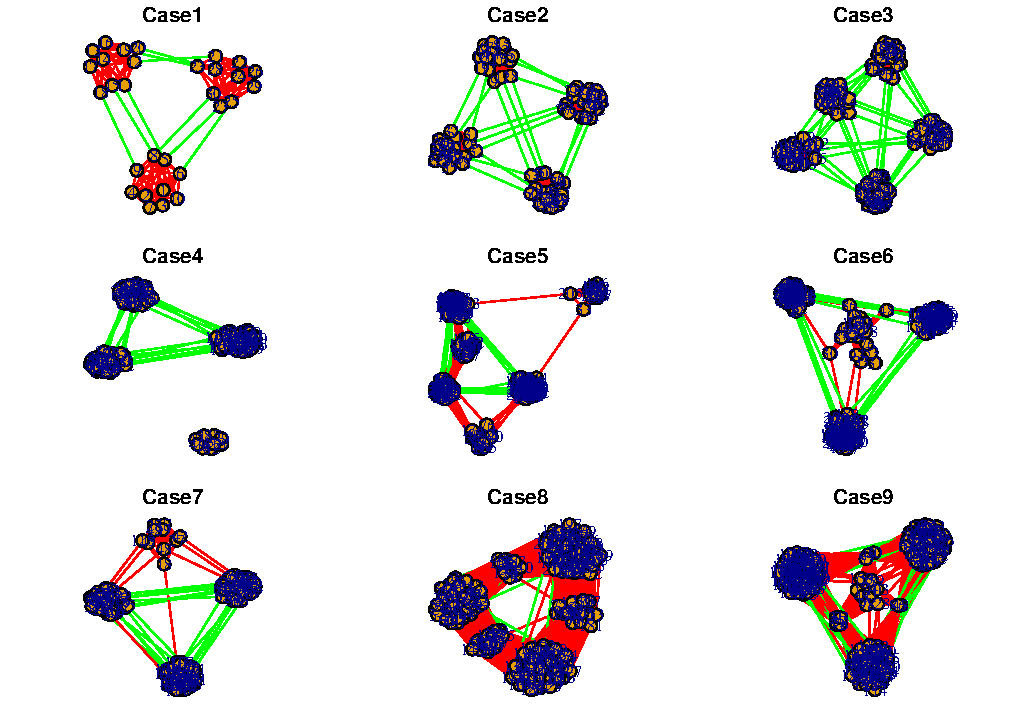
\includegraphics[width=1\textwidth]{Fig1.pdf}
\caption{Graphical illustrations of six synthetic networks.
Nodes that share the common factors are clustered. The cross cluster links are ad-hoc Citations.}
\label{fig:figure1}
\end{figure}

All six networks that are elaborated in scenarios $1$ and $2$ are visualized in Fig.\ref{fig:figure1}.
Notice that the nodes that share the common topics are clustered,
and the cross clustered links are ad-hoc citations.
%ad-hoc links, which connect clusters of papers with $1$ topic, are colored in green.
%Readers can refer the R code provided in $\dots$, for more detailed descriptions on parametric settings for generating networks in Fig\ref{fig:figure1}.

%\subsubsection{Data Generation}
%Following the notation of our paper, each edge $X_{ij}$ follows Bernoulli distribution, whose parameter is parameterized by the probability, $P^{*}_{ij}=\frac{\exp (
%\alpha^{*}+F^{*T}_{i}D^{*}F^{*}_{j} +  S^{*}_{ij})}{1+\exp(\alpha^{*}+F^{*T}_{i}D^{*}F^{*}_{j} +  S^{*}_{ij})}$.
%Here, we describe a procedure on how to set the model parameters, $\alpha^*, S^*, D^*, F^*$, to define the probability $P^*_{ij}$ for generating the random networks in Fig\ref{fig:figure1}.

%\begin{enumerate}
%    \item Generate $\alpha^*$ from uniform distribution supported on $[-11,-10]$. Only for the case $4$, we draw $\alpha^* \sim \text{Unif}[-4,-3]$.

%    \item We assume that the ad-hoc links, induced from non-zero entries of $S^*$ matrix, can complement the latent model
%        the link structure that cannot be explained by common topics.
%        Based on this assumption, we make the ad-hoc links connect the clusters with $K$ distinct topics.

%    \item Each element of diagonal matrix $D^{*}$ is generated from uniform distribution supported on $[19,20]$. (i.e., $D_{ii} \sim \text{Unif}[19,20], \forall 1\leq i \leq K$)

%    \item For factor loading matrix $F^*(\in \mathbb{R}^{K \times n})$, first fill in each row of the matrix with $\floor{\frac{n}{K}}$ ones,
%        and make sure that each column of $F^{*}$ has only one $1$.
%        In last row of $F^*$, fill in the last remaining $n-K\floor{\frac{n}{K}}$ entries with $1$'s.
%        Then, we randomly choose one of columns, and fill that column with ones.
%        Lastly, set $F^*=F^*J$, where $J=I_{n}-\frac{1}{n}\mathbbm{1}\mathbbm{1}^T$.
        %and project the column space of $F$ onto the orthogonal complement subspace of $\mathbbm{1}$ vector by multiplying the aforementioned $J = I_{n}-\frac{1}{n}\mathbbm{1}\mathbbm{1}^T$ to $F$.
%\end{enumerate}

\subsubsection{Choosing the tuning parameters and evaluation criteria}
Choosing a good pair of tuning parameters is an important yet challenging issue in our setting.
Here we present a heuristic procedure for choosing a good pair of tuning parameters $(\gamma,\delta)$.
Following the scree-plot approach in Ji and Jin \cite{ji2016coauthorship}, we plot the largest $15$ eigenvalues of the adjacency matrix $X$, and find an ``elbow'' point where the eigenvalues seem to level off.
An index of the point, which is to the left of this elbow point, is considered as the number of the topics embedded in the network.
(We will denote this number as $\widehat{K}^{\text{Scree}}$.)
We want to note the readers that the scree-plot analysis serves as a good guideline for determining the range of grids to search over.
With the estimate of the number of topics in the network in mind, we record the $\text{rank}(\widehat{L}^{\gamma,\delta})$ and $|\widehat{S}^{\gamma,\delta}|$ for each tuning parameter pair on a given grid.
We need to go through several iterations of this recording procedure to find a proper range of grid, in which we can get $\text{rank}(\widehat{L}^{\gamma,\delta})=\widehat{K}^{\text{Scree}}$
and $10^{-4}|X| \leq |\widehat{S}^{\gamma,\delta}| \leq 10^{-1}|X|$, via adjusting the range of grid for $\gamma$ and $\delta$ repeatedly.
Once we find a grid, which satisfies above constraints, we choose a pair of tuning parameters: %($\gamma^{\text{Heu}},\delta^{\text{Heu}}$):
\[
    (\gamma^{\text{Heu}},\delta^{\text{Heu}}):=
    \big\{(\gamma,\delta): \text{rank}(\widehat{L}^{\gamma,\delta})=\widehat{K}^{\text{Scree}},
    \mbox{mode} |\widehat{S}^{\gamma,\delta}|: \mbox{subject to} 10^{-4}|X| \leq |\widehat{S}^{\gamma,\delta}| \leq 10^{-1}|X| \big\}
\]
One might wonder how traditional model selection methods, such as the Bayes Information Criterion (BIC;\cite{schwarz1978estimating}) and the AIC, work where we recall that BIC and AIC are defined as follows:
\[
\mbox{BIC}(M) = -2  \mathbb{L}_n( \hat{\beta}(M)) + |M| \log \bigg(\frac{n(n-1)}{2}\bigg),
\]
and
\[
\mbox{AIC}(M) = -2  \mathbb{L}_n( \hat{\beta}(M)) + 2|M|.
\]
Here $M$ indicates the current model, which is implicitly understood that the model is obtained from certain tuning parameter pair $(\gamma,\delta)$.
We use $\mathbb{L}_n( \hat{\beta}(M))$ to denote the maximal log-likelihood for a given model $M$,
and $|M|$ is the number of free parameters in $M$, which is determined by the number of non-zeros in $\widehat{S}^{\gamma,\delta}$ and the low-rank matrix $\widehat{L}^{\gamma,\delta}$.
In detail, if we have $\text{rank}(\widehat{L}^{\gamma,\delta})=K$, we can establish the following
\[
|M| = \sum_{i < j}1_{\{S_{ij} \neq 0\}} + n K - \frac{K(K-1)}{2} + 1 ;
\]
since the number of free parameters in $\widehat{L}^{\gamma,\delta}$ is $K$ plus $nK - K(K+1)/2$, which is the number of free parameters in determining $K$ orth-normal vectors.
Additional $1$ in the last term is due to $\hat{\alpha}$.
We want to find a pair $(\gamma,\delta)$, which minimizes BIC($M$) and AIC($M$) as a function of $(\gamma,\delta)$ respectively, where we denote them as follows:
\[
    (\gamma^{BIC},\delta^{BIC}):= \mbox{arg min}_{\gamma, \delta}
    \mbox{BIC}(M),
    \quad
    (\gamma^{AIC},\delta^{AIC}):= \mbox{arg min}_{\gamma, \delta}
    \mbox{AIC}(M)
\]
We evaluate the models that are selected via our heuristic approach, BIC, and AIC by using following four evaluation metrics.

\begin{eqnarray*}
M_1 &=& \mathbbm{1}\big\{\mbox{rank}(\widehat{L}) = \mbox{rank}(L^{*})\big\}, \\
M_2 &=& \frac{\left|\big\{(i,j):i<j:S^{*}_{i,j} \neq0 \quad \& \quad \widehat{S}_{i,j} \neq 0 \big\}\right|}{\left|\big\{(i,j):i<j:S^{*}_{i,j}\neq0\big\}\right|}, \\
M_3 &=& \frac{\left|\big\{(i,j):i<j:S^{*}_{i,j} = 0 \quad \& \quad \widehat{S}_{i,j} \neq 0 \big\}\right|}{\left|\big\{(i,j):i<j:S^{*}_{i,j}=0\big\}\right|}, \\
M_4 &=& \frac{\left|\big\{\mbox{Misclassified Nodes}\big\}\right|}{n},
\end{eqnarray*}
where $M_1$ is a metric on whether the selected model recovers the true low rank structure of network,
$M_2$ evaluates the positive selection rate of the sparse ad-hoc structure in network,
and $M_3$ evaluates the false discovery rate of ad-hoc edges.
$M_4$ calculates the proportion of mis-classified nodes to the entire nodes in the network.
With properly selected tuning parameter, $M_1$ will be 1, $M_2$ will be close to 1, and $M_3$ and $M_4$ will get close to 0.
We present the evaluation results of the six cases via the four criteria, $M_1,M_2,M_3$, and $M_4$ in Table.\ref{tab:table1}.

\subsubsection{Several Observations}
%Given a network data $X$, after fitting the model with a proper pair of tuning parameters, $(\gamma,\delta)$, we need to determine whether node $i$ belongs to $k$th topic or not.
%We apply a simple $k$-means clustering on the fitted $L$ matrix's $K$ eigenvectors.
%For the illustration of performance of our fitted model after applying $k$-means algorithm on three synthetic scenarios, in Fig\ref{fig:figure1}, we plot the coordinates of each rows of first two eigen-vectors on $2$D plane.
%Furthermore, we find one interesting phenomenon.
%Coordinates of each rows from first two eigenvectors of estimated $\widehat{L}$ matrix in our model characterize the clustering behavior of embedded topics reasonably well.
%Our experience shows that with only first two eigenvectors of $\widehat{L}$, we can also cluster the nodes comparably well.
\begin{enumerate}
    \item \textbf{Model Selection.}
    First and foremost, choosing a good pair of tuning parameters is critical when it comes to making a good statistical inference on data.
    As presented in Table.\ref{tab:table1}, both BIC and AIC, which are well known for their model selection consistency in asymptotic setting, appear to under-estimate either the number of topics or the number of ad-hoc links in the networks in our synthetic settings. This may be caused by the fact that these traditional methods take the sample size into account, and therefore penalizes the model complexity too harshly.
    In the heuristic approach, scree-plot plays an important role when it comes to recovering the number of topics, and this strategy leads us to good model selection results for all the six cases considered in two scenarios. (See Fig.\ref{fig:figure2})

    \begin{table}[htbp]
    \centering
    \begin{tabular}{c|ccc|ccc|ccc}
                & \multicolumn{9}{c}{\textbf{Scenario 1}}                                              \\
                \cline{2-10}
                & \multicolumn{3}{c|}{Case 1} & \multicolumn{3}{c|}{Case 2} & \multicolumn{3}{c}{Case 3} \\
                \cline{2-10}
                & Heuristic   & AIC   & BIC  & Heuristic   & AIC   & BIC  & Heuristic   & AIC   & BIC  \\
                \hline
    $M_{1}$   &    1 (3)  &    0 (2)   &  0 (2)  &    1 (4)    &  0 (3)   &  0 (3)  &    1 (5)  &   0 (4)    & 0 (4) \\
    $M_{2}$   &    1     &    0 &      0 &         1    &     1  &    1  &         1    &    1   &   1   \\
    $M_{3}$   &    0     &    0 &      0 &         0    &     0  &    0  &         0    &    0   &   0   \\
    $M_{4}$   &  0  &   $\frac{20}{30}$    &  $\frac{20}{30}$    &   0          &   $\frac{25}{40}$    &   $\frac{25}{30}$   &  0      &  $\frac{30}{30}$     &   $\frac{30}{30}$   \\
                \hline
    \end{tabular}

    \begin{tabular}{c|ccc|ccc|ccc}
                & \multicolumn{9}{c}{\textbf{Scenario 2}}                                              \\
                \cline{2-10}
                & \multicolumn{3}{c|}{Case 4} & \multicolumn{3}{c|}{Case 5} & \multicolumn{3}{c}{Case 6} \\
                \cline{2-10}
                & Heuristic   & AIC   & BIC  &    Heuristic   & AIC   & BIC  & Heuristic   & AIC   & BIC  \\
                \hline
    $M_{1}$   &   1 (3)     &     1 (3)  &  1 (3)    &      1 (3)   &   1 (3)    &  1 (3)    &   1 (3)     &  1 (3)   & 1 (3)   \\
    $M_{2}$   &   $\frac{17}{18}$   &   0    &    0  &   $\frac{17}{18}$     &   0    &  0    &  $\frac{16}{18}$    &   0    &  0    \\
    $M_{3}$   &   0 &     0  &   0   &        0     &    0   &  0    &        0     &   0    & 0 \\
    $M_{4}$   &  0  &   $\frac{20}{120}$    &  $\frac{20}{120}$    &   0          &   $\frac{25}{210}$    &   $\frac{25}{210}$   &  0      &  $\frac{30}{210}$     &   $\frac{30}{210}$   \\
                \hline
    \end{tabular}
    \caption{ For two scenarios, our heuristic method chooses the model with $\widehat{L}$ with true rank, $\widehat{S}$ whose $M_2$ value is close to $1$, and $M_3$ value is close to $0$.
    Also note that it chooses a model whose mis-classification rate is close to $0$.
    A number in the parentheses represents the rank of $\widehat{L}$ estimated from ($\gamma^{\text{Heu}},\delta^{\text{Heu}}$), ($\gamma^{\text{AIC}},\delta^{\text{AIC}}$) and ($\gamma^{\text{BIC}},\delta^{\text{BIC}}$) for each case.}
    \label{tab:table1}
    \end{table}

    \begin{figure}[htbp]
        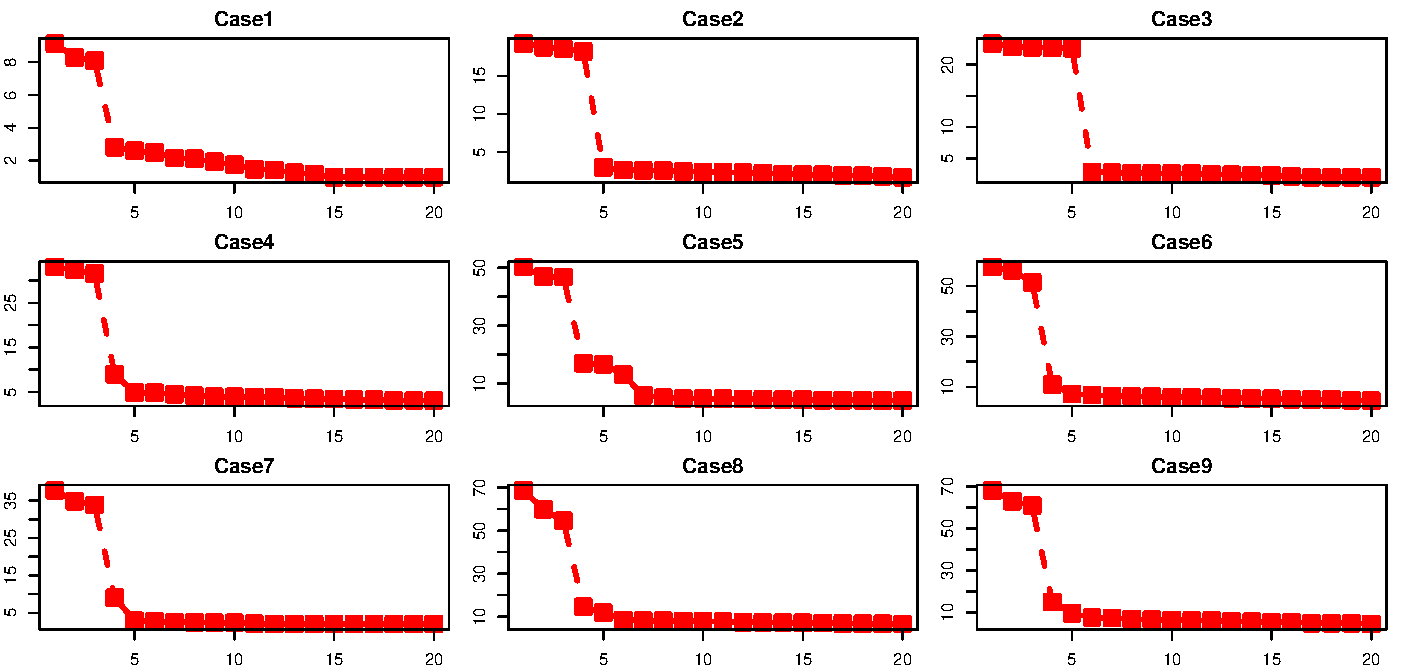
\includegraphics[width=1\textwidth]{Fig2.pdf}
        \caption{ Scree plots for six synthetic Networks.
        $\hat{K}^{\mbox{Scree}}$ recovers the number of topics in the network correctly for all six cases.}
        \label{fig:figure2}
    \end{figure}

    \item \textbf{Node Membership.}
    After fitting the model with a proper pair of tuning parameters, $(\gamma,\delta)$, we need to determine whether the $i$th paper belongs to the $k$th topic or not.
    We apply a simple $k$-means clustering algorithm on the $\widehat{L}$ matrix’s $K$ eigenvectors where $K$ denotes the rank of matrix $\widehat{L}$.
    %(We will denote column-wise concatenation of these $K$ eigenvectors as $\widehat{E}_{K} \in \mathbb{R}^{n\times K}$.)
    For three cases in Scenario $1$, where each paper in the network only has one topic, we confirm that $k$-means algorithm performs well on classifying papers in the network.
    However, in Scenario $2$ where we allow the papers in the network can have more than one topic, naive implementation of $k$-means algorithm entails a problem, since it is not able to afford the overlapped membership of nodes.
    Here, we create a matrix $\widehat{E}_{K}\in \mathbb{R}^{n \times K}$, whose $i$th column corresponds to the $i$th eigenvector of the $\widehat{L}$.
    In order to obtain a sense on how many clusters of papers exist in latent space, we project each row of the $\widehat{E}_{K}$ on the first and second principal components of data matrix $\widehat{E}_{K}$, and plot the projected points on $2$-dimensional plane.
    We count the number of distinct clusters plotted on the plane. Subsequently, we run the $k$-means algorithm on the projected points.
    Refer Table.\ref{tab:table1} and Fig.\ref{fig:figure3} for the references on how this procedure performs on six synthetic cases.

    \begin{figure}[htbp]
    \centering
    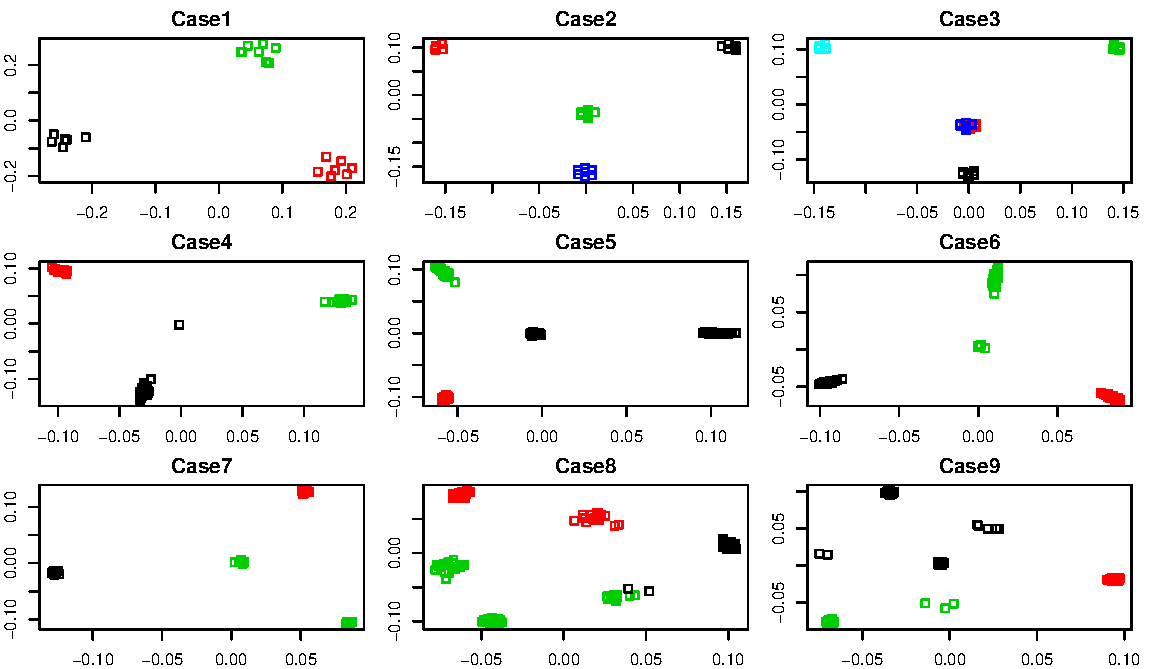
\includegraphics[width=1\textwidth]{Fig3.pdf}
    \caption{ Case $1\sim3$ : Plots of rows from the first two eigenvectors of $\widehat{L}^{\gamma^{\text{Heu}},\delta^{\text{Heu}}}$.
    Case $4 \sim 6$ : Plots of the projected points on the first (X-axis) and second (Y-axis) principal component of the data matrix $\widehat{E}_{K}^{\gamma^{\text{Heu}},\delta^{\text{Heu}}}$. Different colors represent different clusters of papers that $k$-means algorithm assigns.}
    \label{fig:figure3}
    \end{figure}

    %\item \textbf{Scenario $2$ vs. Scenario $3$.}
    %We empirically observe that the number of edges between clusters $\big\{ C_{i,j}:\forall 1 \leq i \neq j \leq K \big\}$ and $\big\{ C_{i}: \forall 1 \leq i \leq K \big\}$ has an effect on their clustering behaviors in latent space. Here $C_{i}$ is used to represent a set of papers on $i$th topic, and $C_{i,j}$ is used to denote a collection of papers that have $i$th and $j$th topics.
    %If we take a look at Fig\ref{fig:figure3}, Case $4$ in second scenario illustrates that it is difficult for us to visually distinguish the papers in $C_{1,2,3}$ and those in $\big\{ C_{i}: \forall 1 \leq i \leq 3 \big\}$ in projected space, whereas they are obviously distinguishable in Case $7$.
    %Unfortunately, we can observe similar phenomenon in Case $5$ and $6$, where the exact separations of clusters $\big\{ C_{i,j}:\forall 1 \leq i \neq j \leq 3 \big\}$ are not made.
    %makes $k$-means algorithm difficult to distinguish the clusters of papers $C_{1,2}, C_{2,3}, C_{1,3}$ and $C_{1,2,3}$ from each other both in Case $5$ and $6$.
    %On the other hand, in third scenario, distinct separations are made between $6$ clusters $C_{1}, C_{2}, C_{3}, C_{1,2}, C_{2,3}, C_{1,3}$ in Case $8$, and between $7$ clusters $C_{1}, C_{2}, C_{3}, C_{1,2}, C_{2,3}, C_{1,3}, C_{1,2,3}$ in Case $9$, so that we can explicitly know the membership of each paper in the network.

    % In fact, this observation is especially helpful for us to understand the behavior of our model with the statisticians’ citation network data, which we are going to explore in the following subsection.
    % In the statisticians’ citation network, we also observe clusters of papers, which have more than $1$ topic, behave similarly with those from the second scenario.

    %\item \textbf{Ad-hoc links.}
    %In our setting, ad-hoc links of synthetic network data are considered as ``across edges'' between clusters $\big\{ C_{i}: \forall 1 \leq i \leq K \big\}$.
    %Our heuristic method works much better than either AIC or BIC in recovering the ad-hoc edges for the $6$ cases in $3$ scenarios.
    %For the three Cases (i.e., Case $2,3,9$) where both AIC and BIC work well, all the pairs of tuning parameters in the grid give the same $|\widehat{S}^{\gamma,\delta}|$.

    %Since indices of non-zero entries of $S^{*}$ are randomly chosen, there might be some indices of positive $S^{*}_{ij}$ entries where $L^{*}_{ij}$ is also positive.
    %In this case, this makes the edges indistinguishable if they come from $S^{*}_{ij}$ or $L^{*}_{ij}$.
    %Some of ``across edges" are also attributed to $\alpha^{*}$, and unfortunately, our algorithm cannot make a difference whether the edge comes from $\alpha^{*}$ or $S^{*}_{ij}$.
    %So the total number of ``across edges'' might not be exactly same as $|S^*|$ as we set in our data generation setting.
\end{enumerate}

%\textbf{Simulation Results}.
%Our goal in this simulation experiment is to check if our model can cluster each nodes into correct communities.
%Also to see if it can separate the ad-hoc links from edges which come from common topics.
%Tuning parameter pairs, $(\gamma,\delta) = (0.01,0.03),(0.004,0.014),(0.003,0.013)$, respectively, give us the desirable results for the three scenarios.
%For first scenario, both $\gamma$ and $\delta$ are searched over $\{0.01,0.02,\dots,0.1\}$.
%For second and third scenarios, parameters are searched over $100$ points, equidistant, from the interval $[0.001,0.01]$ for $\gamma$, and $[0.01,0.02]$ for $\delta$.
%Note that different dynamics of network requires different choices of tuning parameters even the synthetic setting is same, since we are generating the random graph.
%In order to avoid this problem, we set the seeds in our simulation so that the results are reproducible. (Code is provided in $\emph{https://sites.google.com/site/namjoonsuh/publications}$.)
%Fig. \ref{fig:figure1} shows us the result of clustered nodes using $k$-means algorithm on the first $K(=\mbox{rank}(\widehat{L}))$ eigenvectors.
%We plot the rows of first two eigenvectors on the cartesian plane since it visualizes well the clustering behavior of the nodes.
%Our model chooses well the ad-hoc links between clusters of nodes as can be verified in Fig. \ref{fig:figure2}.
%We color the edges in blue whose corresponding elements of estimated $\widehat{S}$ are non-zero, and color the edges in black whose corresponding entries of $\widehat{S}$ are zero.

%\begin{figure}[htbp]
%\begin{center}
%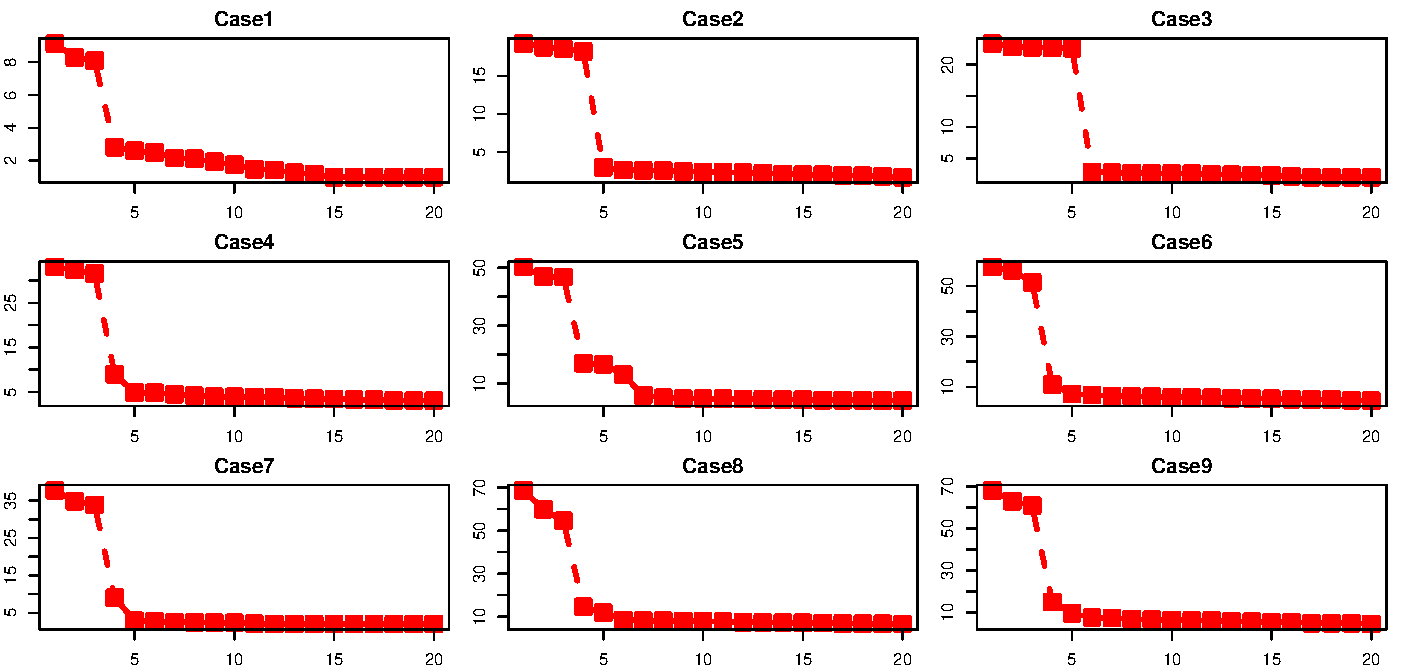
\includegraphics[scale=0.75]{Fig2.pdf}
%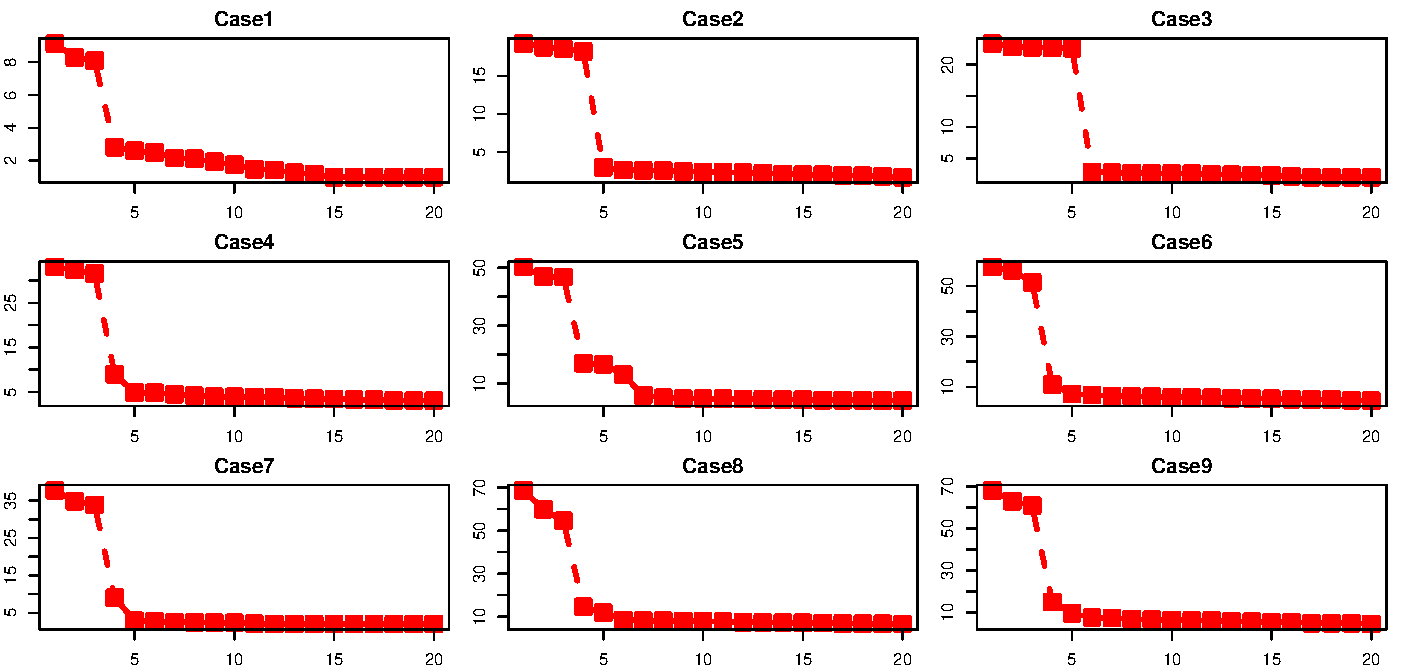
\includegraphics[scale=1,bb=0 0 30 30]{Fig2.pdf}
%\caption{Edges colored with blue correspond to non-zero entries of estimated $\widehat{S}$ matrix.
%For all three cases, our algorithm correctly separates the ``across edges'' from edges coming from low-rank matrix structure.}
%\label{fig:figure2}
%\end{center}
%\end{figure}

\subsection{Citation networks for statisticians}
\label{sec:citation_network}
\begin{figure}[htbp]
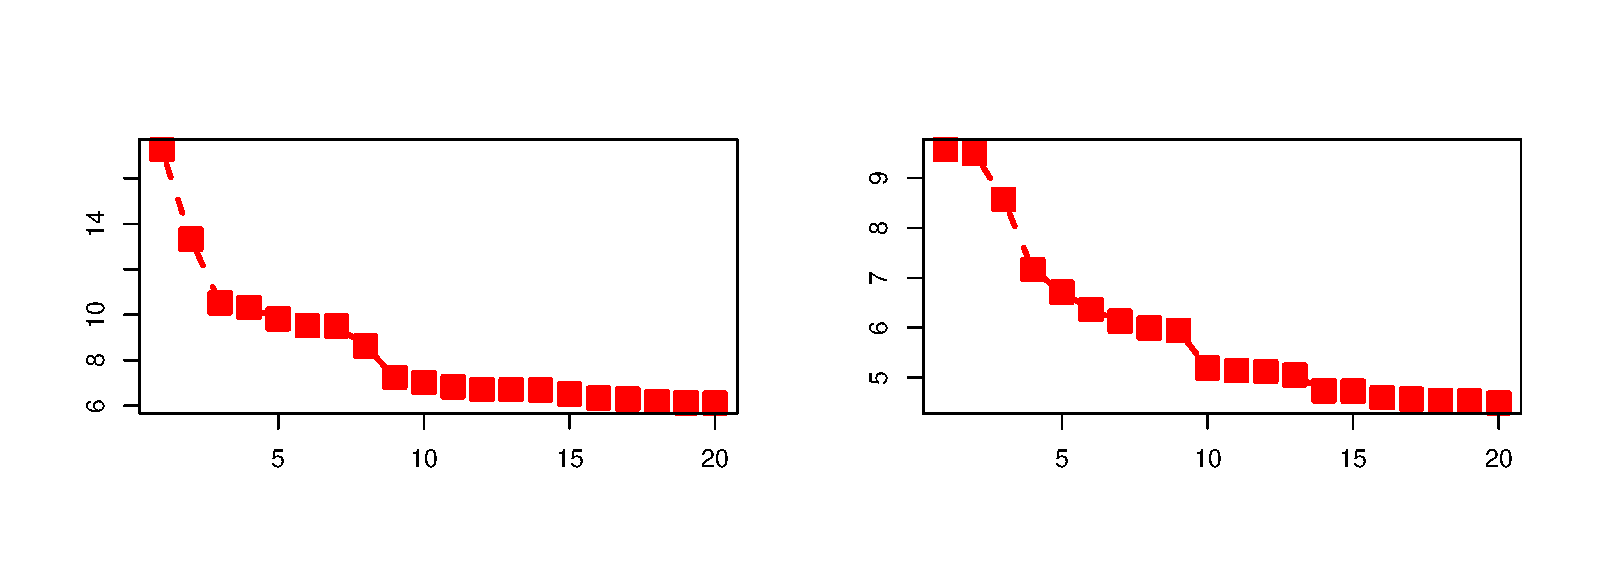
\includegraphics[width=1\textwidth]{Fig4.eps}
\caption{From left to right : Scree plots of the adjacency matrix $X^{\mbox{orig}}$ and $X^{\mbox{sub}}$.}
\label{fig:figure4}
\end{figure}
Recently, Ji and Jin \cite{ji2016coauthorship} published an interesting dataset on citation network of papers from statistics journals.
Specifically, this dataset is based upon all papers published from $2003$ to the first half of $2012$, from the four top statistical journals: Annals of Statistics, Biometrika, Journal of American Statistical Association and Journal of Royal Statistical Society (Series B).
Citational relationships of $3248$ papers are given in the form of adjacency matrix.
In our analysis, we focus our attentions on the papers which have greater than or equal to $10$ citational edges in the network of Ji and Jin \cite{ji2016coauthorship}.
After collecting papers with greater than or equal to $10$ citational edges and eliminating those that have no connecting edges from the rest, we have $232$ papers in total.

We denote the adjacency matrix of these $232$ papers as $X^{\mbox{orig}}$.
Elbow points of the scree plot from $X^{\mbox{orig}}$ may be at the $3$rd, $5$th, or $9$th largest eigenvalue, suggesting that there are from $2$ to $8$ embedded topics in the network. (See Fig. $\ref{fig:figure4}$)
In light of this, we conduct the analysis in two steps:
\begin{enumerate}
    \item First, we assume that the network $X^{\mbox{orig}}$ has $2$ distinct topics and one giant mixed-component, which has a sub-network structure. Under this assumption, we set $\widehat{K}^{\mbox{scree}}$ as $3$, and select a proper model via our heuristic method.
        Then, we perform a $k$-means algorithm on matrix $\widehat{E}_{3}$ treating each row of the matrix as one data point.
        Note that we set the total number of clusters in the network as $3$ when we run the clustering algorithm.
    \item Next, we restrict the network to the giant component ignoring all the edges to/from outside and obtain a subnetwork.
        We denote the adjacency matrix of this subnetwork as $X^{\mbox{sub}}$. We set $\widehat{K}^{\mbox{scree}}$ as $5$, and also select a proper model through the heuristic method.
        Here, we run the $k$-means algorithm on $\widehat{E}_{5}$ setting the number of clusters as $5$.
\end{enumerate}

In the first step, a pair of parameters, $(\gamma^{\text{Heu}},\delta^{\text{Heu}}) = (0.0021094, 0.01913)$, gives us $\widehat{L}^{\mbox{orig}}$ with rank $3$, and $\widehat{S}^{\mbox{orig}}$ with $|\widehat{S}^{\mbox{orig}}|=261$.
We list the first two topics discovered through our analysis. Full list of papers for each community is provided in $https://sites.google.com/site/namjoonsuh/publications$.
\begin{itemize}
    \item Variable selection, which includes $43$ paper.
    \item Multiple Hypothesis Testing, which includes $31$ papers.
\end{itemize}
The first topic is about Variable Selection with high-dimensional data.
The second topic discusses Controlling False Discovery Rate in various statistical settings.
The third group, which consists of $158$ papers, is hard to interpret and appears to have sub-network structures.
For further investigation, we set this group as a giant component in the network, and denote the corresponding network's adjacency matrix as $X^{\mbox{sub}}$.
As aforementioned, we perform a model selection as described in Step $2$, and obtain five sub-communities as follows:

\begin{itemize}
    \item Non-parametric Bayesian Statistics, which includes $15$ papers.
    \item Functional / Longitudinal Data analysis, which includes $16$ papers.
    \item Dimension Reduction, which includes $14$ papers.
    \item High-dimensional covariance estimation, which includes $15$ papers.
    \item Mixed topics, which includes $98$ papers.
\end{itemize}
From the sub-network $X^{\mbox{sub}}$, we got four meaningful topics: Bayesian Statistics, Functional/Longitudinal Data Analysis, Dimension Reduction, and high-dimensional covariance estimation.
Due to the small volume of each community, we could manually check that false discovery for each community is all zero.

Sub-network structure has also a big chunk of papers which we refer it as ``Mixed Topics'' cluster.
Not only could we see the papers with topics on Learning Theory, Non-parametric / Semi-parametric Statistics, Spatial Statistics, Theoretical Machine Learning, which does not seem to belong to any of the five communities listed above, but also we could identify the papers with combinations of two or three topics.
Papers, such as The Bayesian Lasso (T. Park, et al. $2008$), Coordinate-independent sparse sufficient dimension reduction and variable selection (X. Chen, et al. $2010$), are the examples of these papers.
It is also interesting to think about a reason on papers which seem to have obvious membership in one of $5$ communities other than Mixed topic classified as Mixed topic.
For instance, ``On the "degrees of freedom" on the LASSO (H. Zou, et al. $2007$)'' is classified as Mixed Topic paper.
We can simply guess model selection has lots of applications in other topics, so it might cite or have been cited by many papers in other communities.
Actually, out of $19$ citation relationships it has with other papers, $12$ of them came from the relationships with papers from Mixed topics.

Non-zero components of $\widehat{S}^{\mbox{orig}}$ capture the citation relationships among papers that are not attributable to the common topics. The model we select has $261$ sparse edges ($9\%$ of total edges), and all of them are positive edges. In Table \ref{tab:table2}, we provide $15$ pairs of papers that have the largest estimated $\widehat{S}_{ij}^{\mbox{orig}}$. All the $15$ edges come from the pairs of papers from different communities. For instance, the first pair of papers comes from the Functional Analysis community (denoted by \emph{FuncAn}) and Variable Selection $(\emph{VarSel})$ community. $\emph{FuncAn}$ paper cites $\emph{VarSel}$ paper for borrowing a mathematical representation to build a theorem. Though it might appear to be a crucial step for building a theorem in their paper, we cannot say that two papers are closely related in terms of topic. Second pair comes from Multiple Testing (denoted as $\emph{MulT}$) and Variable Selection ($\emph{VarSel}$) community. $\emph{MulT}$ paper briefly mentions about $\emph{VarSel}$ paper in future work section, suggesting a possible way of combining their work and work in $\emph{VarSel}$ paper. And we also observe that as the estimated weight of sparse edges (i.e., $\widehat{S}_{ij}^{\mbox{orig}}$) decreases, the number of pairs of papers that come from Mixed topics community increases.

%\begin{figure}[htbp]
%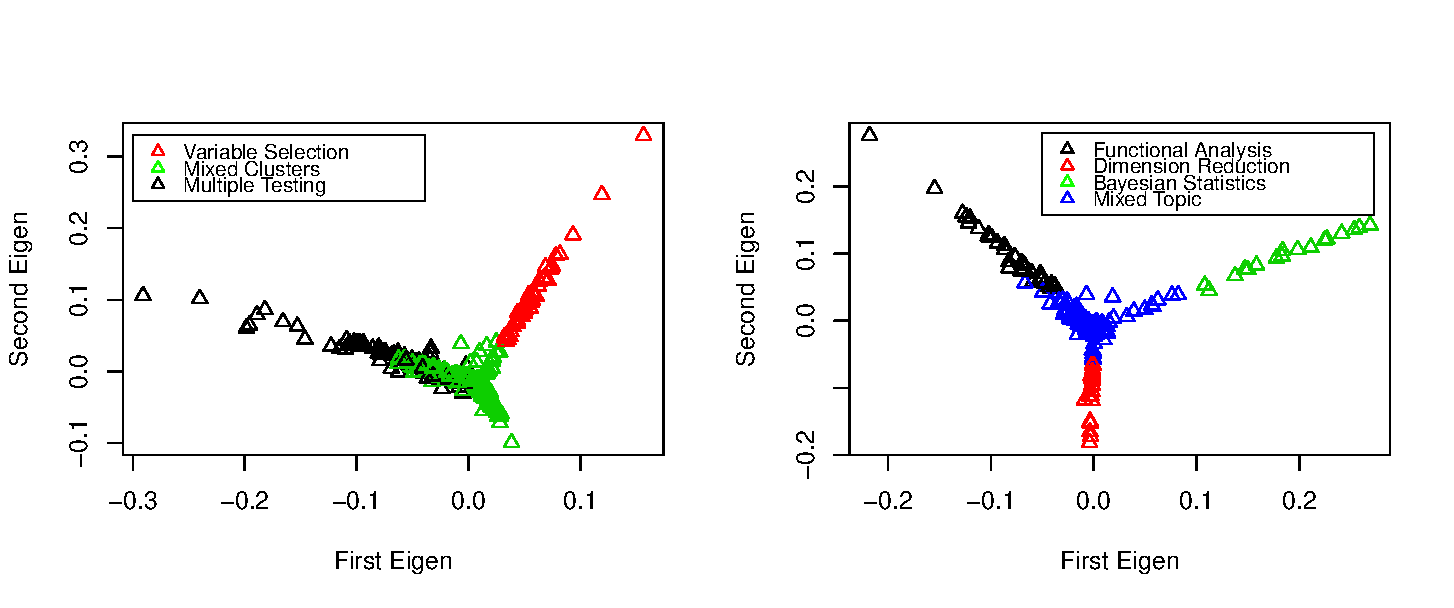
\includegraphics[width=1\textwidth]{Fig5.pdf}
%\caption{Illustration of first two eigenvectors of estimated $\widehat{L}$ matrix for original
%citation network with $543$ papers (left) and sub-network graph (right). We present
%the results of assignment of each paper to each topic via $k$-means algorithm with different colors.}
%\label{fig:figure5}
%\end{figure}

%\begin{landscape}
\begin{table}[htbp]
\centering
\begin{tabular}{lclclcl}\hline
Pair & Community & Title & \\
\hline
1    & FuncAn    & Properties of principal component methods for functional and longitudinal data analysis       & \\
     & VarSel    & Nonconcave penalized likelihood with a diverging number of parameters                         & \\
2    & MulT      & Innovated higher criticism for detecting sparse signals in correlated noise                   & \\
     & VarSel    & Regularized estimation of large covariance matrices & \\
3    & DimRed    & Contour projected dimension reduction & \\
     & VarSel    & Factor profiled sure independence screening & \\
4    & VarSel    & Factor profiled sure independence screening & \\
     & DimRed    & Sliced regression for dimension reduction & \\
5    & VarSel    & Covariance regularization by thresholding & \\
     & MulT      & Adapting to unknown sparsity by controlling the false discovery rate                          & \\
6    & VarSel    & Asymptotic properties of bridge estimators in sparse high-dimensional regression models       & \\
     & Mixed     & Marginal asymptotics for the ``large p small n'' paradigm: with applications to microarray data &  \\
7    & VarSel    & A majorization-minimization approach to Variable Selection using spike and slab priors        & \\
     & Mixed     & Empirical Bayes selection of wavelet thresholds & \\
8    & VarSel    & Spades and mixture models & \\
     & MulT      & Adapting to unknown sparsity by controlling the false discovery rate                          & \\
9    & DimRed    & A constructive approach to the estimation of dimension reduction directions                   & \\
     & VarSel    & Factor profiled sure independence screening & \\
10   & VarSel    & A majorization-minimization approach to variable selection using spike and slab priors        & \\
     & Mixed     & Spike and slab variable selection: Frequentist and Bayesian strategies                        & \\
11   & VarSel    & variable selection in nonparametric additive models & \\
     & Mixed     & Nonparametric estimation of an additive model with a link function                            & \\
12   & Mixed     & Nonparametric inferences for additive models & \\
     & VarSel    & Nonparametric independence screening in sparse ultra-high-dimensional additive models         & \\
13   & Mixed     & Bayesian variable selection in structured high-dimensional covariate spaces with applications in genomics & \\
     & VarSel    & Model selection and estimation in regression with grouped variables                           & \\
14   & VarSel    & The sparsity and bias of the LASSO selection in high-dimensional linear regression            & \\
     & Mixed     & Tests for high-dimensional covariance matrices & \\
15   & FuncAn    & Empirical dynamics for longitudinal data & \\
     & Mixed     & Variable selection in nonparametric varying-coefficient models for analysis of repeated measurements   &       \\\hline
\end{tabular}
\caption{All the $15$ edges come from pairs of papers from different communities. For instance in the first pair, $\emph{FuncAn}$ paper cites $\emph{VarSel}$ paper for borrowing a mathematical representation to build a theorem. But they are not related in terms of topic.}
\end{table}
\label{tab:table2}
%\end{landscape}

\section{Discussion}
\label{sec:Con}

We propose a new combined latent factor and sparse graphical model.
We consider the regularized likelihood by means of $L_1$ and nuclear norm penalties.
The computation of the regularized estimator is facilitated by developing an algorithm based on the alternating direction method of multiplier to optimize a non-smooth and convex objective function.
The proposed method is applied to citation network of statisticians, and the estimated model renders good interpretative power.
Specifically, our analysis on statistician's citation network sheds the new light on the interpretation of dataset.

Nonetheless, there are still several questions remaining to be answered.
First of all, it remains unclear on how to choose the proper tuning parameters.
Classical methods for choosing tuning parameters such as BIC or AIC did not work in our case, since they tend to choose the most parsimonious models.
We also do not have systematic ways to do cross validation in network data.
Not only because it is computationally expensive procedure, but also because if we partition the network data, we can loose fair amount of information on dependent structures among edges.
This problem is also closely related with determining the number of communities in network.
In lieu of using BIC or AIC, our analysis is heavily relying on heuristic approach when choosing the tuning parameter, and during this procedure, we use the screeplot for determining number of communities in network.
Screeplot approach works well in general situation, but it does not necessarily always guarantee the correct estimate of number of communities.
We need a more reliable and theoretically well understood way to determine $K$.

Secondly, we only consider the undirected case which is somewhat unrealistic assumption for citation network in real world, in a sense that it is not usual for two papers to cite each other at the same time.
Since, in our research, we were interested in separating the low rank structure of edges and ad-hoc links in network, we did not take into account the directions of edges in our model.
However, it would be interesting to consider incorporating the directed network into our matrix decomposition framework.

Last but not least, when we assign the memberships of each nodes, we use $k$-means clustering algorithm.
However, $k$-means algorithm turns out that it tends to assign nodes conservatively to each communities.
For example, in Fig.$\ref{fig:figure4}$(left), we can see that bunch of Multiple Testing papers are assigned as Mixed cluster, and in Fig.$\ref{fig:figure4}$(right) also, many papers which should have been classified to among three communities other than mixed topic, have been assigned as Mixed topic community.
This is probably because $k$-means does not allow overlapping membership of each nodes.
It would be interesting to see what happens if we apply some clustering methods which allow the overlapped memberships of nodes in network.

\section{Appendix}
\subsection{Proof of Theorem \ref{Th:th1}}

In the proof, we use the notion of \emph{decomposable regularizer} which is studied at length in the work \cite{negahban2012unified}. Let $(M,M^{\perp})$ denote an arbitrary subspace pair for which component-wise $L_{1}$ norm is decomposable. Throughout the proof, we adopt the convenient short-hand notation on projection of matrix $P$ on subspace $M$ as $P_{M}$. And also note that the proof relies on the following lemma:

\begin{lemma} \label{le:le1}
If a pair of regularization parameters $(\delta,\gamma)$ satisfies condition (\ref{eq:49}), then for $\mathbb{Q}\left(\widehat{\Delta}^L_{B},\widehat{\Delta}^S_{M^\perp}\right)$, we have
\[
    \mathbb{Q}\left(\widehat{\Delta}^L_{B},\widehat{\Delta}^S_{M^\perp}\right) \leq
    \left\|\hat{\Delta}^{\alpha}\mathbbm{1}\mathbbm{1}^T\right\|_{F} +
    3\mathbb{Q}\left(\widehat{\Delta}^{L}_{A},\widehat{\Delta}^{S}_{M}\right)+4 \sum_{j=k+1}^{n} \sigma_{j}(L^{*}) + 4\frac{\gamma}{\delta}
    \left\|S^{*}_{M^\perp}\right\|_{1}
\]
\end{lemma}

\noindent\textbf{Proof of Theorem \ref{Th:th1}}.
\begin{proof}
Since $\widehat{\Theta}$ and $\Theta^{*}$ are optimal minimizer and feasible solution respectively for the convex program (\ref{eq:Modified}), we have
\begin{equation}\label{eq:2}
    h(\widehat{\Theta}) + \delta\|\widehat{L}\|_{*} + \gamma\|\widehat{S}\|_{1} \leq
     h(\Theta^{*}) + \delta\|{L^{*}}\|_{*} + \gamma\|{S}^{*}\|_{1}
\end{equation}

Through the assumption of strong convexity on $h(\Theta)$, and by the Taylor expansion, we can get a following lower bound on the term $h(\widehat{\Theta})-h(\Theta^{*})$ :
\[
h(\widehat{\Theta})-h(\Theta^{*}) \geq
\langle\, \nabla_{\Theta}h(\Theta^{*}),\widehat{\Theta}-\Theta^{*}\rangle\ + \frac{\tau}{2}\|\widehat{\Delta}^{\Theta}\|_{F}^{2}
\]

By rearranging the term in (\ref{eq:2}) and plugging in above inequality relation, we get:

\begin{equation}\label{eq:3}
    \frac{\tau}{2}\|\widehat{\Delta}^{\Theta}\|_{F}^{2} \leq
    -\langle\,\nabla_{\Theta}h(\Theta^{*}),\widehat{\Theta}-\Theta^{*}\rangle\
    + \delta \|L^{*}\|_\ast + \gamma \|S^{*}\|_1
    - \delta \|\widehat{L}\|_\ast - \gamma \|\widehat{S}\|_1
\end{equation}

Here, we introduce another notation, for any pair of positive tuning parameters $(\delta,\gamma)$ which is defined as the weighted combination of the two regularizers :
\[
\mathbb{Q}(L,S)   := \|L\|_{*} + \frac{\gamma}{\delta}\|S\|_1
\]
Through the definition of $\mathbb{Q}$, we can rewrite (\ref{eq:3}) as follows:
\begin{equation}\label{eq:4}
    \frac{\tau}{2}\|\widehat{\Delta}^{\Theta}\|_{F}^{2} \leq
    -\langle\,\nabla_{\Theta}h(\Theta^{*}),\widehat{\Theta}-\Theta^{*}\rangle\
    + \delta \mathbb{Q}(L^{*},S^{*}) - \delta \mathbb{Q}(\widehat{\Delta}^L + L^{*},\widehat{\Delta}^S + S^{*})
\end{equation}

According to Agarwal et al \cite{agarwal2012noisy}'s second element of lemma 1,
the difference $\mathbb{Q}(L^*,S^*)- \mathbb{Q}(\widehat{\Delta}^L + L^{*},\widehat{\Delta}^S + S^{*})$ is upper-bounded by

\begin{equation}\label{eq:5}
    \mathbb{Q}(\widehat{\Delta}^L_{A},\widehat{\Delta}^S_{M}) - \mathbb{Q}(\widehat{\Delta}^L_{B},\widehat{\Delta}^S_{M^\perp})
    +2 \sum_{j=k+1}^{n} \sigma_{j}(L^*) + 2\frac{\gamma}{\delta}\|S^*_{M^\perp}\|_{1}
\end{equation}

First, we want to control upper bound of the term $-\langle\,\nabla_{\Theta}h(\Theta^{*}),\widehat{\Theta}-\Theta^{*} \rangle\,$
in (\ref{eq:4}).
\begin{align}
-\langle\,\nabla_{\Theta}h(\Theta^{*}),\widehat{\Theta}-\Theta^{*} \rangle\  \nonumber
&=\langle\, \frac{1}{n} (X - P^*), \widehat\Delta^{\alpha\mathbbm{1}\mathbbm{1}^T} + \widehat\Delta^{L} + \widehat\Delta^{S} \rangle\ \\ \nonumber
&\leq \frac{1}{n} \|X - P^*\|_{op}(\|\widehat{\Delta}^{\alpha}\mathbbm{1}\mathbbm{1}^T\|_\ast + \|\widehat{\Delta}^{L}\|_\ast) +  \frac{1}{n} \|X - P^*\|_{\infty}\|\widehat{\Delta}^{S}\|_{1} \\ \nonumber
&\leq \frac{1}{n} \|X - P^*\|_{op}(\|\widehat{\Delta}^{\alpha}\mathbbm{1}\mathbbm{1}^T\|_{F} + \|\widehat{\Delta}^{L}_{A}\|_\ast + \|\widehat{\Delta}^{L}_{B}\|_\ast) +
\frac{1}{n} \|X - P^*\|_{\infty}(\|\widehat{\Delta}^{S}_{M}\|_{1} +
\|\widehat{\Delta}^{S}_{M^{\perp}}\|_{1}) \\
&\leq \frac{\delta}{2}(\|\hat{\Delta}^{\alpha}\mathbbm{1}\mathbbm{1}^T\|_{F} + \|\widehat{\Delta}^{L}_{A}\|_\ast + \|\widehat{\Delta}^{L}_{B}\|_\ast) + \frac{\gamma}{2}(\|\widehat{\Delta}^{S}_{M}\|_{1} +
\|\widehat{\Delta}^{S}_{M^{\perp}}\|_{1})  \label{eq:10}
\end{align}

Combining the inequalities (\ref{eq:5}) and (\ref{eq:10}), we can obtain the upper bound of RHS in (\ref{eq:4}) as follows:

\begin{equation}
    \frac{\tau}{2}\|\widehat{\Delta}^{\Theta}\|_{F}^{2} \leq
    \frac{\delta}{2}\|\hat{\Delta}^{\alpha}\mathbbm{1}\mathbbm{1}^T\|_{F} +
    \frac{3\delta}{2}\mathbb{Q}(\widehat{\Delta}^L_{A},\widehat{\Delta}^S_{M})
    +2 \delta \sum_{j=k+1}^{n} \sigma_{j}(L^*) + 2\gamma \|S^*_{M^\perp}\|_{1}
    \label{eq:11}
\end{equation}

Second, we wish to control the lower bound of the term  $\frac{\tau}{2}\|\widehat{\Delta}^{\Theta}\|_{F}^{2}$ with respect to $\hat{\Delta}^{\alpha},\widehat{\Delta}^{L},\widehat{\Delta}^{S}$.
\begin{align}
\|\widehat{\Delta}^{\Theta}\|_{F}^{2}  \nonumber
&= \|\widehat{\Theta}-\Theta^{*} \|_{F}^{2} \\ \nonumber
&= \|\widehat\Delta^{\alpha\mathbbm{1}\mathbbm{1}^T} + \widehat\Delta^{L} + \widehat\Delta^{S}\|_{F}^{2} \\ \nonumber
&= \|\hat{\Delta}^{\alpha}\mathbbm{1}\mathbbm{1}^T\|_{F}^{2} + \|\widehat{\Delta}^{L}+\widehat{\Delta}^{S}\|_{F}^{2} +
2 \langle\, \widehat\Delta^{L} + \widehat\Delta^{S} ,\hat{\Delta}^{\alpha}\mathbbm{1}\mathbbm{1}^T \rangle\ \\
&=  \|\hat{\Delta}^{\alpha}\mathbbm{1}\mathbbm{1}^T\|_{F}^{2} + \|\widehat{\Delta}^{L}\|_{F}^{2} + \|\widehat{\Delta}^{S}\|_{F}^{2} +
2 \langle\, \widehat\Delta^{L} + \widehat\Delta^{S} ,\hat{\Delta}^{\alpha}\mathbbm{1}\mathbbm{1}^T \rangle\ +
2 \langle\, \widehat\Delta^{L}, \widehat\Delta^{S} \rangle\  \label{eq:12}
\end{align}

We want to get the further lower bound on trace inner product terms,
$ \langle\, \widehat\Delta^{L} + \widehat\Delta^{S} ,\hat{\Delta}^{\alpha}\mathbbm{1}\mathbbm{1}^T \rangle\ $, $ \langle\, \widehat\Delta^{L}, \widehat\Delta^{S} \rangle\ $. To control the first trace inner product term, we use the relation $\widehat{\Delta}^{L}\mathbbm{1}=0$, apply the definition of dual norm on inner product term, apply triangular inequality on $\hat{\Delta}^\alpha$, and lastly we apply the constraint imposed on $|\alpha|$ stated in Assumption \ref{Ass:2}.

\begin{align}
    | \langle\, \widehat\Delta^{L} + \widehat\Delta^{S} ,\hat{\Delta}^{\alpha}\mathbbm{1}\mathbbm{1}^T\rangle\ | \nonumber
    &= | \langle\,\widehat\Delta^{S},\hat{\Delta}^{\alpha}\mathbbm{1}\mathbbm{1}^T\rangle\ | \\ \nonumber
    &\leq \|\hat{\Delta}^{\alpha}\mathbbm{1}\mathbbm{1}^T \|_{\infty} \|\widehat{\Delta}^{S}\|_1 \\ \nonumber
    &\leq (|\hat{\alpha}|+|\alpha^{*}|)\|\widehat{\Delta}^{S}\|_1\\
    &\leq 2C\kappa\|\widehat{\Delta}^{S}\|_1  \label{eq:13}
\end{align}

To control the term $ \langle\, \widehat\Delta^{L}, \widehat\Delta^{S} \rangle\ $, we first apply the definition of dual norm on trace inner product term, then apply triangular inequality on $\widehat{\Delta}^{L}$ and spikiness condition.

\begin{align}
    | \langle\, \widehat\Delta^{L}, \widehat\Delta^{S} \rangle\ | \nonumber
    &\leq \|\widehat{\Delta}^{L}\|_{\infty} \|\widehat{\Delta}^{S}\|_1\\ \nonumber
    &\leq (\|\widehat{L}\|_{\infty} + \|L^{*}\|_{\infty})
    \|\widehat{\Delta}^{S} \|_{1}\\
    &\leq \big(\frac{2\kappa}{n}\big)\|\widehat{\Delta}^{S} \|_{1} \label{eq:14}
\end{align}

We can combine the inequality (\ref{eq:12}), (\ref{eq:13}) and (\ref{eq:14}). Then applying the assumption on regularization parameter $\gamma$, and the fact $\|\widehat{\Delta}^{L}\|_{\ast}\geq0$ sequentially, we can get,

\begin{align}
    \frac{\tau}{2}\|\widehat{\Delta}^{\Theta}\|_{F}^{2}  \nonumber
    &\geq \frac{\tau}{2} \|\hat{\Delta}^{\alpha}\mathbbm{1}\mathbbm{1}^T\|_{F}^{2} + \frac{\tau}{2} \|\widehat{\Delta}^{L}\|_{F}^{2} + \frac{\tau}{2} \|\widehat{\Delta}^{S}\|_{F}^{2}
    - 2\kappa\tau(\frac{Cn+1}{n})\|\widehat{\Delta}^{S}\|_{1} \\ \nonumber
    &\geq \frac{\tau}{2} \|\hat{\Delta}^{\alpha}\mathbbm{1}\mathbbm{1}^T\|_{F}^{2} + \frac{\tau}{2} \|\widehat{\Delta}^{L}\|_{F}^{2} + \frac{\tau}{2} \|\widehat{\Delta}^{S}\|_{F}^{2} - \frac{\gamma}{2}\|\widehat{\Delta}^{S}\|_{1}\\
    &\geq \frac{\tau}{2} \|\hat{\Delta}^{\alpha}\mathbbm{1}\mathbbm{1}^T\|_{F}^{2} + \frac{\tau}{2} \|\widehat{\Delta}^{L}\|_{F}^{2} + \frac{\tau}{2} \|\widehat{\Delta}^{S}\|_{F}^{2} - \frac{\delta}{2} \mathbb{Q}(\widehat{\Delta}^L,\widehat{\Delta}^S) \label{eq:26}
\end{align}

By combining the relations (\ref{eq:11}) and (\ref{eq:26}), applying triangular inequality, $\mathbb{Q}(\widehat{\Delta}^L,\widehat{\Delta}^S)\leq \mathbb{Q}(\widehat{\Delta}^L_{A},\widehat{\Delta}^S_{M}) + \mathbb{Q}(\widehat{\Delta}^L_{B},\widehat{\Delta}^S_{M^{\perp}})$, and rearranging the term, we can get following inequality,
\[
    \frac{\tau}{2} \|\hat{\Delta}^{\alpha}\mathbbm{1}\mathbbm{1}^T\|_{F}^{2} + \frac{\tau}{2} \|\widehat{\Delta}^{L}\|_{F}^{2} + \frac{\tau}{2} \|\widehat{\Delta}^{S}\|_{F}^{2} \\
    \leq \frac{\delta}{2} \|\hat{\Delta}^{\alpha}\mathbbm{1}\mathbbm{1}^T\|_{F} +
    2\mathbb{Q}(\widehat{\Delta}^L_{A},\widehat{\Delta}^S_{M}) +  \frac{\delta}{2} \mathbb{Q}(\widehat{\Delta}^L_{B},\widehat{\Delta}^S_{M^\perp}) +
    2 \delta \sum_{j=k+1}^{n} \sigma_{j}(L^{*}) + 2\gamma
    \|S^{*}_{M^\perp}\|_{1}
\]

Further, by plugging in Lemma 1 to get an upper bound on  $\mathbb{Q}(\widehat{\Delta}^L_{B},\widehat{\Delta}^S_{M^\perp})$, we can rewrite the above inequality as follows:
\begin{align}
    \frac{\tau}{2} \|\hat{\Delta}^{\alpha}\mathbbm{1}\mathbbm{1}^T\|_{F}^{2} + \frac{\tau}{2} \|\widehat{\Delta}^{L}\|_{F}^{2} + \frac{\tau}{2} \|\widehat{\Delta}^{S}\|_{F}^{2} -
    \frac{\delta}{2} \|\hat{\Delta}^{\alpha}\mathbbm{1}\mathbbm{1}^T\|_{F}
    \leq
    \frac{7\delta}{2}\mathbb{Q}(\hat{\Delta}^L_{A},\hat{\Delta}^S_{M}) + 4 \delta \sum_{j=k+1}^{n} \sigma_{j}(L^*) + 4\gamma \|S^*_{M^\perp}\|_{1}  \label{eq:42}
\end{align}
Noting that $\widehat{\Delta}^{L}_{A}$ has rank at most 2$k$ and that $\widehat{\Delta}^{S}_{M}$ lies in the model space $M$, we find that
\begin{align}
    \nonumber
    \delta\mathbb{Q}(\widehat{\Delta}^L_{A},\widehat{\Delta}^S_{M})
    \leq \sqrt{2k}\delta\|\widehat{\Delta}^L_{A}\|_{F} + \Psi(M)\gamma\|\widehat{\Delta}^S_M\|_{F}\\
    \leq \sqrt{2k}\delta\|\widehat{\Delta}^L\|_{F} + \Psi(M)\gamma\|\widehat{\Delta}^S\|_{F}  \label{eq:43}
\end{align}
Here $\Psi(M)$ measures the compatibility between Frobenius norm and component-wise $L_{1}$ regularizer, where $M$ is an arbitrary subset of matrix indices of cardinality at most s.
\[
    \Psi(M):=\sup\limits_{U\in M,U\neq0}\frac{\|U\|_{1}}{\|U\|_{F}}
\]
Using Cauchy-Schwarz inequality, we can easily check the quantity $\Psi(M)$ is bounded by at most $\sqrt{s}$. Plugging in the relation ($\ref{eq:43}$) into ($\ref{eq:42}$) and rearranging the term relevant with  $e^{2}(\hat{\alpha}\mathbbm{1}\mathbbm{1}^T,\widehat{L},\widehat{S})$ yield the claim.
\end{proof}


\subsection{Proof of Lemma \ref{le:le1}}

\begin{proof}
Through the application of basic inequality by using optimality of $\widehat{\Theta}$ and feasibility of $\Theta^{*}$ to convex program (\ref{eq:1}), we have
\begin{equation}
    h(\widehat{\Theta}) - h(\Theta^{*})
    \leq \delta \mathbb{Q}(L^{*},S^{*}) - \delta \mathbb{Q}(\widehat{\Delta}^L + L^{*},\widehat{\Delta}^S + S^{*})
\end{equation}
By using convexity of $h(\Theta)$, we can write
\begin{align}
    h(\widehat{\Theta})-h(\Theta^{*}) &\geq
    \langle\, \nabla_{\Theta}h(\Theta^{*}),\widehat{\Theta}-\Theta^{*}\rangle\ \nonumber \\
    &= - \langle\,\frac{1}{n} (X-P^{*}), \hat{\Delta}^{\alpha}\mathbbm{1}\mathbbm{1}^T + \widehat{\Delta}^{L} + \widehat{\Delta}^{S} \rangle\ \nonumber \\
    &\geq -\frac{1}{n} \|X - P^*\|_{op}(\|\hat{\Delta}^{\alpha}\mathbbm{1}\mathbbm{1}^T\|_\ast + \|\widehat{\Delta}^{L}\|_\ast) +  \frac{1}{n} \|X - P^*\|_{\infty}\|\widehat{\Delta}^{S}\|_{1} \nonumber \\
    &\geq -\frac{\delta}{2}(\|\hat{\Delta}^{\alpha}\mathbbm{1}\mathbbm{1}^T\|_F + \|\widehat{\Delta}^{L}_{A}\|_\ast + \|\widehat{\Delta}^{L}_{B}\|_\ast) - \frac{\delta}{2} (\|\widehat{\Delta}^{S}_{M}\|_{1} +
    \|\widehat{\Delta}^{S}_{M^\perp}\|_{1}) \label{eq:27}
\end{align}

One more round of application on Agarwal et al \cite{agarwal2012noisy}'s second element of lemma 1,
we can get an upper bound of difference $\mathbb{Q}(L^*,S^*)- \mathbb{Q}(\widehat{\Delta}^L + L^{*},\widehat{\Delta}^S + S^{*})$ as follows:

\begin{equation} \label{eq:28}
    \mathbb{Q}(\widehat{\Delta}^L_{A},\widehat{\Delta}^S_{M}) - \mathbb{Q}(\widehat{\Delta}^L_{B},\widehat{\Delta}^S_{M^\perp})
    +2 \sum_{j=k+1}^{n} \sigma_{j}(L^*) + 2\frac{\gamma}{\delta}\|S^*_{M^\perp}\|_{1}
\end{equation}

By combining relations (\ref{eq:27}) and (\ref{eq:28}), we can get the upper bound of $\mathbb{Q}(\widehat{\Delta}^L_{B},\widehat{\Delta}^S_{M^\perp})$ :
\begin{align*}
    \mathbb{Q}(\widehat{\Delta}^L_{B},\widehat{\Delta}^S_{M^\perp}) \leq
    \|\hat{\Delta}^{\alpha}\mathbbm{1}\mathbbm{1}^T\|_{F} +
    3\mathbb{Q}(\widehat{\Delta}^{L}_{A},\widehat{\Delta}^{S}_{M})+4 \sum_{j=k+1}^{n} \sigma_{j}(L^{*}) + 4\frac{\gamma}{\delta}
    \|S^{*}_{M^\perp}\|_{1}
\end{align*}



\end{proof}

%\nocite{*}
\bibliography{References}


%\backmatter

\end{document}




